% ICML 2027 submission — EDA-LiveFlow-Bench
% 双盲投稿：使用 [submitted] 选项（匿名）
% camera-ready 时改为 [accepted] 并填作者信息
%
% 需要的 style 文件（从 icml.cc 下载 Author Kit 2027）：
%   icml2027.sty, icml2027.bst, fancyhdr.sty
% 放在本目录下即可编译。
%
% 编译：pdflatex main && bibtex main && pdflatex main && pdflatex main
%
% 结构遵循 ML 会议惯例（参考 SWE-bench, ICLR 2024）：
%   Intro → Benchmark → Harness → Experiments → Analysis → Related Work → Conclusion → Ethics/Reproducibility
%   References → Appendix A/B/C
% 注意：Related Work 放在结果之后（非 IEEE 期刊惯例的 §2）。

\documentclass{article}

% ICML 2027 Author Kit 尚未发布；当前使用仓库自带的 icml2026.sty/.bst（接口一致）。
% 拿到 2027 kit 后：把 icml2026.sty/.bst 换成 icml2027.*，并同步改本行与 \bibliographystyle。
\usepackage{hyperref}
\usepackage{icml2026}

% 基础包
\usepackage{amsmath,amssymb}
\usepackage{graphicx}
\usepackage{booktabs}
\usepackage{algorithm}
\usepackage{algorithmic}
\usepackage{xspace}
\usepackage{multirow}
\usepackage{tabularx}

% 宏定义
\newcommand{\bench}{EDA-LiveFlow-Bench\xspace}
\newcommand{\mode}{design\_flow\xspace}
\newcommand{\eg}{e.g.,\xspace}
\newcommand{\ie}{i.e.,\xspace}
\newcommand{\etal}{\textit{et al.}\xspace}
% 任务总数（唯一事实源）：每轮只改这一行
% 2026-11-13 r454 DEBT-fix: downline duplicate-trace PatternSpeedAnalyze-001 (r451 re-claimed session 0kv56 already used by PatStatSpeed-001 11/07) => A:256->255, sum 1197->1196. r453 was 1197.
% 2026-11-13 r455 造题: +VerilogPowerPinConsist-001 (ykb7a) => A:255->256, sum 1196->1197.
% 2026-11-13 r456 造题: +OdtErrScan-001 (gbzuy) => A:256->257, sum 1197->1198.
% 2026-11-13 r458 造题: +FailReportModuleFilter-001 (ofg4y) => A:257->258, sum 1198->1199.
% 2026-11-13 r461 造题: +NetlistHierTracer-001 (1236h, verification) => A:260->261, sum 1210->1211.
% 2026-11-13 r463 造题: +SvPackedFlatten-001 (vjcll, digital) => A:261->262.
% 2026-11-13 r464 造题: +RegrCheckMacroMap-001 (udmg8, verification) => A:262->263. \Ntasks 1211->1218 (catch-up A262/263 + B/C/D increments; truth A263+B289+C310+D356=1218).
% 2026-11-13 r490 造题: B 1113-pool 切换后 r485-r490 连产 6 case => B:289->291. r615/r616 D 1113-pool 2 case => D:356->357. A/C 不变. \Ntasks 1218->1221 (truth A263+B291+C310+D357=1221).
% 2026-11-13 r466 造题: +CaselistPerlDriverGen-001 (gaekj, digital) => A:263->264. \Ntasks 1221->1222 (truth A264+B291+C310+D357=1222).
% 2026-11-13 r467 造题: +GpioPortRefactor-001 (1ckh3, digital) => A:264->265. \Ntasks 1222->1223 (truth A265+B291+C310+D357=1223).
% 2026-11-13 r468 造题: +FmDontVerifyGen-001 (5bngi, verification) => A:265->266. \Ntasks 1223->1224 (truth A266+B291+C310+D357=1224).
% 2026-11-13 r469 造题: +NetlistIncludeRewrite-001 (suz5p, digital) => A:266->267. B/C/D catch-up (B293/C313/D358). \Ntasks 1224->1231 (truth A267+B293+C313+D358=1231).
% 2026-11-13 r470 造题: +RandStimVecFix-001 (qhx2f, digital) => A:267->268. B/C/D catch-up (B294/C314/D359). \Ntasks 1231->1235 (truth A268+B294+C314+D359=1235).
% 2026-11-13 r471 造题: +XrunLogStatusCheck-001 (rawgv, digital) => A:268->269. \Ntasks 1235->1236 (truth A269+B294+C314+D359=1236).
% 2026-11-13 r473 造题: +NetlistPadDriverTrace-001 (i3u9r, digital) => A:269->270. \Ntasks 1236->1237 (truth A270+B294+C314+D359=1237).
% 2026-11-13 r474 造题: +StdcellFamilyRefMatch-001 (8mrkr, digital) => A:270->271. \Ntasks 1237->1238 (truth A271+B294+C314+D359=1238).
% 2026-11-13 r475 造题: +PowerIsoCellRtlGen-001 (yx1e1, digital) => A:271->272. \Ntasks 1238->1239 (truth A272+B294+C314+D359=1239).
% 2026-11-13 r476 造题: +StaStepDriverGen-001 (3aslp, pnr_signoff) => A:272->273. B/C/D catch-up (B299/C319/D363). \Ntasks 1239->1254 (truth A273+B299+C319+D363=1254).
% 2026-11-13 r477 造题: +NetlistHierModuleExtract-001 (fjenb, digital) => A:273->274. \Ntasks 1254->1255 (truth A274+B299+C319+D363=1255).
% 2026-11-13 r478 造题: +SignalXrefMap-001 (u54d9, verification) => A:274->275. B/C/D catch-up (B301/C321/D365). \Ntasks 1255->1262 (truth A275+B301+C321+D365=1262).
% 2026-11-13 r479 造题: +BjobsDupCwdDetect-001 (6c5ev, eda_other) => A:275->276. \Ntasks 1262->1263 (truth A276+B301+C321+D365=1263).
% 2026-11-14 r480 造题: +NetlistSigNameRename-001 (on45q, digital) => A:276->277. \Ntasks 1263->1264 (truth A277+B301+C321+D365=1264).
% 2026-11-14 r483 造题: +SpfRcSummaryGen-001 (7oclp, pnr_signoff) => A:277->278. B/C/D catch-up (B302/C324/D369). \Ntasks 1264->1273 (truth A278+B302+C324+D369=1273).
% 2026-11-14 r485 造题: +SpfNetCapDiff-001 (eyiut, pnr_signoff) => A:278->279. C/D catch-up (C324->326/D369->371). \Ntasks 1273->1278 (truth A279+B302+C326+D371=1278).
\newcommand{\Ntasks}{1324}
% 2026-11-14 r533 sync: A282+B312+C349+D381=1324 (A +2 since r531: r532 VerilogPatternMerge-001 + r533 VpsRegrCfgGen-001; B +1, C +2, D +3 catch-up). Truth verified via committed EDA-Flow-Bench jsonl wc -l.
% 2026-11-14 r531 sync: A280+B311+C347+D378=1316 (C +4 since r522 catch-up; A unchanged, 0-case A-core blocked scan stale + fresh files evaporated 5/5 NOFILE).
% 2026-11-14 r522 sync: A280+B311+C343+D378=1312 (C +1 since r521; A unchanged this round, 0-case broad-filter fresh-peek 6/6 REJECT, quality exhaustion freshly evidenced).
% 2026-11-14 r521 sync: A280+B311+C342+D378=1311 (D +1 since r520; A unchanged this round, 0-case broad-filter exhaustion 37th round freshly evidenced).
% 2026-11-14 r520 sync: A280+B311+C342+D377=1310 (C +2 since r518; A unchanged this round, 0-case broad-filter exhaustion).
% Lite 集：从 Full 集中按领域均衡 + 难度校准 + 可释放性三维度筛选的子集，用于日常评测与外部复现
\newcommand{\LiteSet}{500}
% 冻结评测快照：2026-11-09 run_batch_20261109_171201 = 696 runs
%   （62 PASS + 558 FAIL + 70 ERROR + 6 ABSENT；见 §4 与附录 B）
%   ⚠️ 所有"结果/通过率"句子必须用 \Neval{}，不要用 \Ntasks{}，两者不是同一个数：
%   \Ntasks 是不断增长的 Full 集规模，\Neval 是本文实际评测的冻结快照。
\newcommand{\Neval}{696}

% 图表路径
\graphicspath{{figures/}}

% ===== 标题与作者（ICML 2026+ 接口：twocolumn + icmlauthorlist）=====
\begin{document}

\twocolumn[
  \icmltitle{EDA-LiveFlow-Bench: Benchmarking LLM Agents on Real-World Circuit Design Flow Orchestration}

  \icmltitlerunning{EDA-LiveFlow-Bench}

  % 双盲：不写真实作者；样式在非 accepted 模式下不显示
  \begin{icmlauthorlist}
    \icmlauthor{Anonymous Submission}{anon}
  \end{icmlauthorlist}

  \icmlaffiliation{anon}{Anonymous Institution}

  \icmlcorrespondingauthor{Anonymous Submission}{anonymous@example.org}

  \icmlkeywords{EDA, LLM agents, benchmark, design flow, tool orchestration}

  \vskip 0.3in
]
\printAffiliationsAndNotice{}

% ===== 主体章节（按 ML 会议惯例排序）=====
\begin{abstract}
Existing LLM benchmarks for EDA target single-function code generation (RTLLM, VerilogEval) or open-source flow repair (FlowFixer-EDA), but none evaluate the end-to-end \emph{orchestration} of multi-step design flows with live commercial EDA tools.
% 现有的面向 EDA 的 LLM 基准测试只关注单函数代码生成（RTLLM、VerilogEval）或开源流程修复（FlowFixer-EDA），尚无一个基准真正评估在真实商业 EDA 工具上对多步设计流进行端到端"编排"的能力。
We present \bench, a benchmark of \textbf{\Ntasks{} tasks} (Full set) across \textbf{13 EDA domains}---from schematic/netlist to SPICE simulation, physical verification, and digital synthesis---each derived from \emph{real coding-agent traces} of IC design engineers in a production environment, with a \textbf{\LiteSet{}-task Lite set} released for efficient external evaluation.
% 我们提出 \bench，包含 \textbf{\Ntasks{} 个任务}（Full 集），覆盖 \textbf{13 个 EDA 领域}——从原理图/网表到 SPICE 仿真、物理验证和数字综合——每一个任务都来源于真实生产环境中 IC 设计工程师使用编程智能体的交互轨迹；同时发布 \textbf{\LiteSet{} 个任务的 Lite 集}用于高效的外部评测。
Each task requires the agent to produce a deliverable package (\texttt{submit.zip}) by orchestrating remote EDA tools through an MCP bridge, scored against $\geq 8$ executable assertions with a \texttt{PreToolUse} hook that prevents answer leakage.
% 每个任务要求智能体通过 MCP 网桥调用远程 EDA 工具，最终产出一个交付件包（\texttt{submit.zip}）；判分基于不少于 8 条可执行断言，并通过 \texttt{PreToolUse} 钩子防止答案泄露。
On a frozen \Neval{}-run evaluation snapshot, a single frontier backbone (DeepSeek-V4-Pro) reaches only \textbf{10.0\% Pass@1} (62/620 decided runs)---versus 76.5\% on single-script EDA benchmarks---showing that multi-step flow orchestration is qualitatively harder than isolated code generation.
% 在冻结的 \Neval{}-run 评测快照上，单一前沿骨干（DeepSeek-V4-Pro）仅取得 \textbf{10.0\% Pass@1}（62/620 已判定 run）——而单脚本 EDA 基准上为 76.5\%——表明多步流程编排比孤立的代码生成在本质上更为困难。
Failure analysis attributes the gap to \emph{tool-chain grounding depth}: the highest-passing domain (pnr\_signoff, 20.8\%) exceeds the lowest (physical\_verify and layout\_aether, both 2.9\%) by a factor of $7.1\times$ (a descriptive point estimate; the two confidence intervals overlap), and the lowest-passing domains are precisely those demanding the deepest live-tool interaction (DRC/LVS runs, GUI-driven layout editing).
% 失败分析把差距归因于"工具链接地深度"：通过率最高的领域（pnr\_signoff，20.8\%）与最低的领域（physical\_verify 与 layout\_aether，均为 2.9\%）相差 7.1 倍（描述性点估计；两个置信区间重叠），而通过率最低的领域恰好是需要最深实时工具交互（DRC/LVS 运行、GUI 驱动的版图编辑）的领域。
\end{abstract}

\section{Introduction}
\label{sec:introduction}

% 第 1 段：问题动机 — 设计流编排是工程师最耗时的工作
Circuit design is less about writing individual components and more about \emph{orchestrating design flows}: a chip tape-out requires traversing schematic capture, SPICE simulation, layout generation, DRC/LVS physical verification, parasitic extraction, timing signoff, and dozens of tool-to-tool handoffs. Each EDA tool is a closed system; where tools refuse to interoperate, the only recourse is hand-written glue---a Tcl driver, a SKILL wrapper, a Python script parsing a simulation log---precisely the intent-to-code synthesis at which LLMs excel. This reframes EDA workflow automation as \emph{agentic flow orchestration}: a coding agent that can call live EDA tools, inspect their outputs, and iteratively refine a deliverable across multiple steps.
% 电路设计的核心不在于编写单个组件，而在于"编排设计流"：一次芯片 tape-out 需要穿越原理图录入、SPICE 仿真、版图生成、DRC/LVS 物理验证、寄生参数提取、时序签核，以及数十次工具间衔接。每件 EDA 工具都是封闭系统；当工具之间无法互操作时，唯一的办法就是手写粘合代码——一段 Tcl 驱动、一个 SKILL 包装、一个解析仿真日志的 Python 脚本——而这正是 LLM 所擅长的"意图到代码"综合。这把 EDA 工作流自动化重新定义为"智能体式流程编排"：一个能够调用真实 EDA 工具、检视其输出、并跨多步迭代改进交付件的编程智能体。

% 第 2 段：现有 benchmark 的缺口
Existing LLM benchmarks for EDA fall into two categories, neither of which captures this orchestration challenge. \emph{Code-generation benchmarks} (RTLLM~\cite{lu2024rtllm}, VerilogEval~\cite{liu2023verilogeval}) evaluate single-function RTL generation from natural language---one module, one testbench, no tool interaction. \emph{Flow-repair benchmarks} (FlowFixer-EDA~\cite{dong2026flowfixer}, EDA-FlowBench) evaluate diagnosing and patching failures in open-source RTL-to-GDS runs---but only on open-source tools (Yosys, OpenROAD), not the commercial EDA ecosystem where most engineers work. Neither evaluates the \emph{end-to-end agentic loop}: read a task description, call live EDA tools through an MCP bridge, inspect execution results, and produce a complete deliverable package. Software engineering benchmarks like SWE-bench~\cite{jimenez2024swebench} test this loop for GitHub issues, but no equivalent exists for EDA design flows.
% 现有的面向 EDA 的 LLM 基准可分为两类，但都未捕捉到这一编排挑战。"代码生成类基准"（RTLLM、VerilogEval）评估从自然语言到单函数 RTL 的生成——一个模块、一个测试台、无工具交互。"流程修复类基准"（FlowFixer-EDA、EDA-FlowBench）评估在开源 RTL-to-GDS 流程中诊断并修复失败——但仅限于开源工具（Yosys、OpenROAD），而非大多数工程师实际使用的商业 EDA 生态。两者都没有评估"端到端智能体回路"：读取任务描述、通过 MCP 网桥调用真实 EDA 工具、检视执行结果、并产出完整的交付件包。软件工程类基准如 SWE-bench 针对 GitHub issue 测试了这一回路，但在 EDA 设计流领域尚无对应物。

% 第 3 段：我们的方法 — 从真实用户轨迹构建 benchmark
We present \bench, built from an unprecedented data source: \textbf{real user interaction traces} of 268 engineers using the Cline~\cite{cline2026} coding agent across 42 workstations in a production IC design environment. Each task in \bench{} is derived from an actual multi-turn session where an engineer used an LLM agent to solve a real design-flow problem---ranging from generating a SPICE deck for a sense amplifier, to writing a DRC rule-check script for a DRAM layout, to automating netlist connectivity tracing for a mixed-signal block. We systematically mined 698 hosts, identified 1{,}511 candidate sessions (match-count $\geq 30$ EDA-keyword hits), and curated \Ntasks{} tasks across 13 EDA domains, each with $\geq 8$ executable assertions and a reference deliverable.
% 我们提出 \bench，其数据来源前所未有：来自生产 IC 设计环境中 42 台工作站上 268 位工程师使用 Cline 编程智能体的真实交互轨迹。\bench{} 中的每个任务都源自一段真实的多轮会话——工程师曾用 LLM 智能体解决一个真实的设计流问题，从为灵敏放大器生成 SPICE 仿真卡，到为 DRAM 版图编写 DRC 规则检查脚本，再到为混合信号模块自动化网表连通性追踪。我们系统性地扫描了 698 台主机，筛出 1,511 个候选会话（EDA 关键词命中数 $\geq 30$），并在 13 个 EDA 领域中精心整理了 \Ntasks{} 个任务，每个任务配有不少于 8 条可执行断言和一份参考交付件。

% 第 4 段：评测协议 + 防泄题
Each task follows a unified \mode{} contract: the agent receives a task brief and input assets, must orchestrate remote EDA tools (on a dedicated EDA server) through an MCP~\cite{lee2025autoeda} bridge, and produce a deliverable package (\texttt{submit.zip}). Scoring is execution-based---a judge unpacks the deliverable and runs reference assertions against it---with a \texttt{PreToolUse} hook that blocks the agent from accessing the answer key (check.py, reference/), ensuring the pass rate reflects genuine agentic capability rather than answer leakage.
% 每个任务遵循统一的 \mode{} 契约：智能体接收任务简述与输入附件，必须通过 MCP 网桥调用远程 EDA 工具（位于专用 EDA 服务器），并产出交付件包（\texttt{submit.zip}）。判分基于执行——判分器解包交付件并运行参考断言——同时配合 \texttt{PreToolUse} 钩子，阻止智能体访问答案（check.py、reference/），确保通过率反映真实的智能体能力而非答案泄露。

% 第 5 段：核心发现
We evaluate a single frontier LLM agent (DeepSeek-V4-Pro) under a controlled Cline harness and obtain a striking result: it achieves only \textbf{10.0\% Pass@1} (62/620 decided runs) on the frozen \Neval{}-run evaluation, far below the 76.5\% reported on single-script EDA benchmarks~\cite{zhu2026edascript}. The gap is domain-dependent: standardized-flow domains where the deliverable is largely a script or tcl template (pnr\_signoff 20.8\%, characterization 19.2\%, eda\_other 18.2\%) pass at roughly twice the overall rate, while domains that require deep live-tool interaction---physical verification (DRC/LVS runs, 2.9\%) and Aether layout editing (2.9\%)---pass at the bottom of the range. We hypothesise that this ordering is explained by \emph{tool-chain grounding depth}---the number of live EDA tool interactions needed to produce a correct deliverable---and we separate what is measured (the domain ordering, the outcome mix, and the per-run trace mechanics) from what remains an untested hypothesis (that grounding depth dominates model scale).
% 我们在受控的 Cline 框架下评测单一前沿 LLM 智能体（DeepSeek-V4-Pro），得到一个引人注目的结果：它在冻结的 \Neval{}-run 评测上仅取得 \textbf{10.0\% Pass@1}（62/620 已判定 run），远低于单脚本 EDA 基准上报告的 76.5\%。
% 该差距随领域而变：交付件主要为脚本或 tcl 模板的标准化流程领域（pnr_signoff 20.8\%、characterization 19.2\%、eda_other 18.2\%）的通过率约为整体的两倍，而需要深度实时工具交互的领域——物理验证（DRC/LVS 运行，2.9\%）与 Aether 版图编辑（2.9\%）——通过率垫底。
% 我们假设这一排序可由"工具链接地深度"——产出正确交付件所需的真实 EDA 工具交互次数——解释；并把"已测量"（领域排序、结果构成、逐 run 轨迹机制）与"仍属未检验假设"（接地深度压过模型规模）明确区分开。

% 第 6 段：贡献
\noindent\textbf{Contributions.}
% \noindent\textbf{贡献。}
\begin{itemize}
    \item \textbf{Benchmark.} \bench: \Ntasks{} tasks from real user traces, 13 EDA domains, execution-based scoring with anti-leakage protocol (Section~\ref{sec:benchmark}).
    % \textbf{基准。} \bench：来自真实用户轨迹的 \Ntasks{} 个任务，覆盖 13 个 EDA 领域，执行式判分加防泄题协议（第~\ref{sec:benchmark}~节）。
    \item \textbf{Evaluation.} First systematic evaluation of an LLM agent on multi-step EDA design-flow orchestration with live commercial tools, revealing a 10.0\% Pass@1 ceiling (62/620 decided runs) on the frozen \Neval{}-run snapshot and a $7.1\times$ point-estimate spread between the best and weakest domain (pnr\_signoff 20.8\% vs.\ physical\_verify/layout\_aether 2.9\%) (Section~\ref{sec:experiments}).
    % \textbf{评测。} 首次系统性地评估 LLM 智能体在真实商业工具上的多步 EDA 设计流编排能力，在冻结的 \Neval{}-run 快照上揭示 10.0\% 的通过率天花板（62/620 已判定 run），以及最好/最弱领域间 7.1 倍的点估计跨度（pnr\_signoff 20.8\% vs.\ physical\_verify/layout\_aether 2.9\%）（第~\ref{sec:experiments}~节）。
    \item \textbf{Analysis.} A failure taxonomy with run-level anchors (PASS 62 / FAIL 558 / ERROR 70 / ABSENT 6), an explicit protocol for per-run attribution, and a trace-anatomy study of 47 archived runs showing where agent effort actually goes (median 26.5 tool calls, 41.2\% through the MCP bridge) (Section~\ref{sec:analysis}).
    % \textbf{分析。} 带 run 级锚点的失败分类法（PASS 62 / FAIL 558 / ERROR 70 / ABSENT 6）、逐 run 归因的显式协议，以及对 47 份归档轨迹的解剖研究，说明智能体的投入实际流向何处（中位 26.5 次工具调用，41.2\% 走 MCP 网桥）（第~\ref{sec:analysis}~节）。
\end{itemize}

\section{Benchmark Construction}
\label{sec:benchmark}

\subsection{Data Source: Real User Interaction Traces}
\label{sec:data-source}
% \subsection{数据来源：真实用户交互轨迹}

Unlike synthetic benchmarks constructed by task authors, \bench{} is built from \emph{real user interaction traces}---actual multi-turn sessions where IC design engineers used a coding agent~\cite{cline2026} to solve design-flow problems in a production environment. We systematically scanned engineering workstations, identified sessions containing EDA-related tool interactions, and curated tasks from the most representative ones.
% 与由任务作者构造的合成基准不同，\bench{} 构建于"真实用户交互轨迹"之上——即 IC 设计工程师在生产环境中使用编程智能体解决设计流问题的真实多轮会话。我们系统性地扫描了工程工作站，识别出包含 EDA 相关工具交互的会话，并从中挑选最具代表性的部分整理为任务。

\textbf{Scan pipeline.} We grep session files for EDA-keyword matches (hspice, spectre, calibre, virtuoso, aether, innovus, pt\_shell, dc\_shell, netlist, schematic, etc.) and rank sessions by \emph{match-count} (mc)---the number of lines hitting any EDA keyword. A two-stage prefilter (rule-based + 0.8B LLM classifier) filters non-design-flow sessions (Q\&A, permission-denied, tool-not-found), with 0\% rejection rate on the mc $\geq 30$ pool---confirming that high-mc sessions are almost universally genuine EDA work.
% \textbf{扫描流程。} 我们对会话文件进行 EDA 关键词匹配（hspice、spectre、calibre、virtuoso、aether、innovus、pt\_shell、dc\_shell、netlist、schematic 等），并按"匹配计数"(mc)——命中任意 EDA 关键词的行数——对会话排序。一个两级预筛器（基于规则 + 0.8B LLM 分类器）过滤掉非设计流会话（问答、权限被拒、工具未找到），在 mc $\geq 30$ 池上拒绝率为 0\%——印证了高 mc 会话几乎全都是真实的 EDA 工作。

\textbf{Trace attribution.} Each task records \texttt{trace\_source} (host, user, session\_file, session\_msgs, real\_task\_summary), enabling trace-back to the original engineer's workflow. User identifiers are preserved (not hashed) for reproducibility, with only API keys/tokens masked.
% \textbf{轨迹溯源。} 每个任务记录 \texttt{trace\_source}（主机、用户、会话文件、会话消息数、真实任务摘要），可回溯至原始工程师的工作流。用户标识保留（不做哈希）以保证可复现性，仅对 API 密钥/令牌进行脱敏。

\subsection{Task Schema: The \mode{} Contract}
\label{sec:task-schema}
% \subsection{任务模式：\mode{} 契约}

All \Ntasks{} tasks follow a unified \mode{} contract (Table~\ref{tab:task-schema}):
% 所有 \Ntasks{} 个任务遵循统一的 \mode{} 契约（表~\ref{tab:task-schema}）：

\begin{itemize}
    \item \textbf{Prompt}: A natural-language task description derived from the real user's intent, reformulated to be self-contained (no assumed context from the original session).
    % \textbf{提示词}：源自真实用户意图的自然语言任务描述，改写为自包含形式（不依赖原始会话的上下文）。
    \item \textbf{Assets}: Input files (RTL fragments, simulation logs, technology files, spec documents) that the agent reads locally.
    % \textbf{附件}：智能体在本地读取的输入文件（RTL 片段、仿真日志、工艺文件、规格文档）。
    \item \textbf{Entry point}: \texttt{outputs/submit.zip}---the agent must write deliverable files under \texttt{outputs/} and the harness packages them into \texttt{submit.zip}.
    % \textbf{入口点}：\texttt{outputs/submit.zip}——智能体须将交付件写入 \texttt{outputs/}，由评测框架打包为 \texttt{submit.zip}。
    \item \textbf{Test}: A two-parameter check function \texttt{check(deliverable, workdir)} that unpacks the deliverable and runs $\geq 8$ assertions.
    % \textbf{测试}：一个双参判分函数 \texttt{check(deliverable, workdir)}，解包交付件并运行不少于 8 条断言。
    \item \textbf{No lang/host}: Unlike single-script benchmarks, the task does not specify a language or runtime---the agent must infer the appropriate tool chain from the task description.
    % \textbf{不指定语言/主机}：与单脚本基准不同，任务不指定编程语言或运行时——智能体须从任务描述自行推断合适的工具链。
\end{itemize}

\begin{table}[ht]
\centering
\small
\caption{Task schema comparison: single-script (EDA-Scripting-Bench) vs.\ \mode{} (\bench).}
% \caption{任务模式对比：单脚本（EDA-Scripting-Bench）vs.\ \mode{}（\bench）。}
\label{tab:task-schema}
\begin{tabularx}{\linewidth}{@{}lXX@{}}
\toprule
 & \textbf{Single-script} & \textbf{Design-flow (\bench)} \\
\midrule
Entry point & function return value & \texttt{outputs/\allowbreak submit.zip} \\
Tool interaction & single \texttt{run\_code} & multi-step MCP orchestration \\
Deliverable & one code file & multi-file package \\
Assertions & function-level & deliverable-level ($\geq 8$) \\
Lang/host specified & yes (pyAether/\allowbreak SKILL/\allowbreak Tcl) & no (agent infers) \\
Steps & 1--3 tool calls & 5--20+ tool calls \\
\bottomrule
\end{tabularx}
\end{table}

\subsection{Domain Coverage}
\label{sec:domain-coverage}
% \subsection{领域覆盖}

\bench{} spans 13 EDA design domains (Figure~\ref{fig:domain-distribution}), organized into four area groups:
% \bench{} 覆盖 13 个 EDA 设计领域（图~\ref{fig:domain-distribution}），按方向组织为四个领域组：
% 注：不再在正文写死的组内任务数——living build 每轮都在增长（2026-11-10: \Ntasks{}），
% 写死的组计数会立刻过期；精确的 shard 计数见附录~\ref{sec:benchmark-details}。

\begin{itemize}
    \item \textbf{Digital front}: digital, verification, pnr\_signoff, eda\_other
    % \textbf{数字前端}：digital、verification、pnr\_signoff、eda\_other
    \item \textbf{SPICE / characterization}: spice\_sim, characterization
    % \textbf{SPICE / 表征}：spice\_sim、characterization
    \item \textbf{Physical / layout}: physical\_verify, layout\_aether, layout\_virtuoso, pg\_layout
    % \textbf{物理 / 版图}：physical\_verify、layout\_aether、layout\_virtuoso、pg\_layout
    \item \textbf{Schematic / netlist / analog}: schematic\_netlist, waveform, analog\_context
    % \textbf{原理图 / 网表 / 模拟}：schematic\_netlist、waveform、analog\_context
\end{itemize}

The living benchmark currently holds \Ntasks{} curated cases (the \emph{Full set}); all results in
Sections~\ref{sec:experiments}--\ref{sec:analysis} are reported on a \emph{frozen
evaluation snapshot} of \Neval{} runs (2026-11-09), whose domain mix is shown in
Figure~\ref{fig:domain-distribution}. Freezing the snapshot is what makes the
per-domain table, the failure analysis and any future re-run comparable.
% 活基准当前含 \Ntasks{} 个已整理案例（\emph{Full 集}）；第~\ref{sec:experiments}--\ref{sec:analysis}~节的
% 全部结果都报告在一个 \emph{冻结的评测快照}（2026-11-09，\Neval{} 个 run）上，其领域构成见
% 图~\ref{fig:domain-distribution}。冻结快照是逐域表格、失败分析与将来重跑可比性的前提。

\textbf{Lite set.} To enable efficient daily evaluation and external reproduction,
we release a \emph{Lite set} of \LiteSet{} tasks selected from the Full set along
three dimensions: (i) \emph{domain balance}---stratified sampling across all 13
EDA domains so that no single domain exceeds 15\% of the Lite set; (ii)
\emph{difficulty calibration}---retaining tasks whose reference pass rate under
the frozen snapshot falls in the 5--25\% band, so that the Lite set is neither
trivially easy nor uniformly impossible; and (iii) \emph{releaseability}---tasks
whose underlying design assets have been approved for external publication are
prioritized, so that the Lite set can be fully released without confidentiality
constraints. The Lite set is intended as the default evaluation surface for new
agents; the Full set remains available for organizations that can access the
full asset inventory.
% \textbf{Lite 集}。为支持高效的日常评测与外部复现，我们从 Full 集中按三个维度筛选
% \LiteSet{} 个任务作为 \emph{Lite 集}：(i) 领域均衡——在 13 个 EDA 领域上分层抽样，
% 任一领域不超过 Lite 集的 15\%；(ii) 难度校准——保留冻结快照下参考通过率在 5--25\% 区间的任务，
% 使 Lite 集既非 trivial 也非 uniformly impossible；(iii) 可释放性——优先选择底座设计资产
% 已获对外发布批准的任务，使 Lite 集可在无保密约束下完整发布。Lite 集是新智能体评测的默认入口；
% Full 集仍可供能访问完整资产清单的组织使用。

The distribution reflects real engineering practice: schematic/netlist and SPICE simulation dominate (analog/mixed-signal design accounts for the largest share), while digital synthesis and PNR signoff are comparatively underrepresented---not because they are less important, but because digital engineers use coding agents less frequently (they work in IDEs and command-line flows). We revisit the implications of this imbalance in Section~\ref{sec:threats}.
% 该分布反映了真实工程实践：原理图/网表与 SPICE 仿真占主导（模拟/混合信号设计占比最大），而数字综合与 PNR 签核相对偏少——并非因为它们不重要，而是因为数字工程师较少使用编程智能体（他们多在 IDE 和命令行流程中工作）。我们在第~\ref{sec:threats}~节重新讨论这种失衡的影响。

\begin{figure}[ht]
\centering
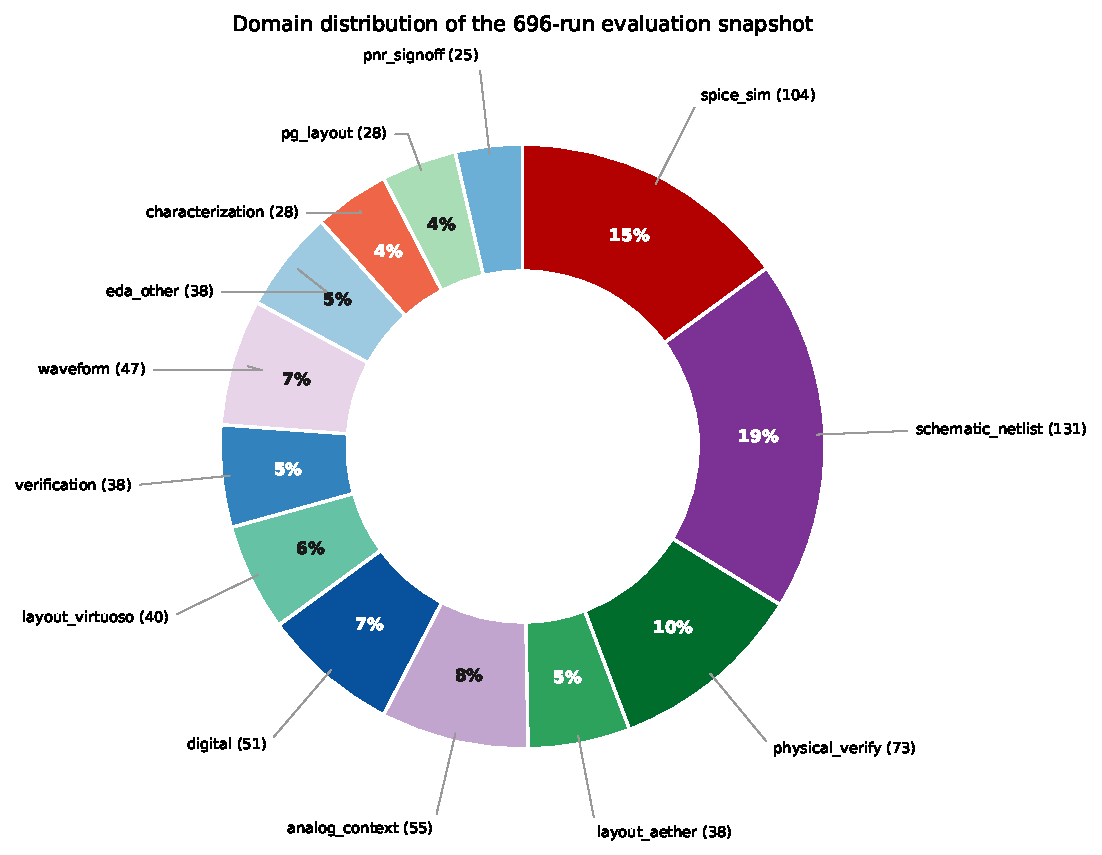
\includegraphics[width=\linewidth]{figures/domain_pie.pdf}
\caption{Domain distribution of the frozen \Neval{}-run evaluation snapshot across 13 EDA domains, colored by area group (counts include the 70 ERROR and 6 ABSENT runs of Table~\ref{tab:full-domain-results}). The donut layout keeps small slices legible; percentages are shown for slices $\geq 4\%$.}
% \caption{冻结的 \Neval{} 个 run 评测快照在 13 个 EDA 领域上的分布，按领域组着色（含表~\ref{tab:full-domain-results} 的 70 个 ERROR 与 6 个 ABSENT）。环形布局使小切片也可读；占比 $\geq 4\%$ 的切片显示百分比。}
\label{fig:domain-distribution}
\end{figure}

\subsection{Evaluation Metric and Protocol}
\label{sec:eval-protocol}
% \subsection{评测指标与协议}

\textbf{Pass@1.} One trace per task: the agent may iterate within the trace (multiple tool calls) but is never restarted. A 2400-second timeout per task. A task passes iff \emph{all} $k \geq 8$ assertions in the reference \texttt{check.py} hold.
% \textbf{Pass@1。} 每个任务一次轨迹：智能体可在该轨迹内迭代（多次工具调用），但不会被重启。每个任务超时 2400 秒。当且仅当参考 \texttt{check.py} 中所有 $k \geq 8$ 条断言全部成立时，该任务判为通过。

\textbf{Execution-based scoring.} The reference judge unpacks \texttt{submit.zip} into a fresh workdir and runs assertions against the deliverable, using only Python standard library (no EDA license required for judging). Each assertion is documented in the \texttt{test\_rationale} field as ``k assertions: (1), (2), ...'' for interpretability.
% \textbf{执行式判分。} 参考判分器将 \texttt{submit.zip} 解包到一个全新的工作目录，并针对交付件运行断言，仅使用 Python 标准库（判分无需 EDA 许可证）。每条断言以"k 条断言：(1)、(2)、……"的形式记录在 \texttt{test\_rationale} 字段中，便于可解释性。

The full evaluation harness---including the agent system, MCP bridge, anti-leakage hook, and judge implementation---is described in Section~\ref{sec:harness} (main text) and Appendix~\ref{sec:experimental-details} (implementation details).
% 完整的评测框架——包括智能体系统、MCP 网桥、防泄题钩子和判分器实现——在正文第~\ref{sec:harness}~节和附录~\ref{sec:experimental-details}~节（实现细节）中描述。

\section{Agent System and Evaluation Harness}
\label{sec:method}

\subsection{System Under Test: Cline Agent}
\label{sec:cline-agent}
% \subsection{被测系统：Cline 智能体}

The system under test (SUT) is Cline v3.0.51~\cite{cline2026}, an open-source coding agent that provides:
% 被测系统（SUT）为 Cline v3.0.51，一个开源编程智能体，提供：
\begin{itemize}
    \item \textbf{File tools}: \texttt{read\_file}, \texttt{write\_to\_file} for local workspace access.
    % \textbf{文件工具}：\texttt{read\_file}、\texttt{write\_to\_file}，用于本地工作区访问。
    \item \textbf{MCP bridge}: EDA tools are exposed via the \texttt{eda\_flow} MCP server (port 18891), providing \texttt{open\_session}, \texttt{run\_commands}, \texttt{run\_code}, \texttt{read\_file}, \texttt{write\_file}, \texttt{list\_files}.
    % \textbf{MCP 网桥}：EDA 工具通过 \texttt{eda\_flow} MCP 服务器（端口 18891）暴露，提供 \texttt{open\_session}、\texttt{run\_commands}、\texttt{run\_code}、\texttt{read\_file}、\texttt{write\_file}、\texttt{list\_files}。
    \item \textbf{Thinking modes}: \texttt{low}/\texttt{medium}/\texttt{high} reasoning budget (we use \texttt{low} as default).
    % \textbf{思考模式}：\texttt{low}/\texttt{medium}/\texttt{high} 三档推理预算（默认用 \texttt{low}）。
    \item \textbf{Auto-approve}: All tool calls are auto-approved (no human-in-the-loop).
    % \textbf{自动批准}：所有工具调用自动批准（无人工介入）。
\end{itemize}

\subsection{Evaluation Harness Architecture}
\label{sec:harness}
% \subsection{评测框架架构}

The evaluation harness (\texttt{run\_one.sh} / \texttt{run\_batch.sh}) implements the following pipeline (Figure~\ref{fig:pipeline}):
% 评测框架（\texttt{run\_one.sh} / \texttt{run\_batch.sh}）实现了如下流水线（图~\ref{fig:pipeline}）：

\begin{enumerate}
    \item \textbf{Deploy hook}: Copy \texttt{PreToolUse} hook to \texttt{\textasciitilde/.cline/hooks/}, configure scope to the evaluation workdir root.
    % \textbf{部署钩子}：将 \texttt{PreToolUse} 钩子拷贝到 \texttt{\textasciitilde/.cline/hooks/}，把作用范围配置为评测工作目录根。
    \item \textbf{Prepare workdir}: Create a fresh workdir, copy task assets (input files, task brief), verify no answer leakage (check.py/reference/ absent).
    % \textbf{准备工作目录}：创建全新工作目录，拷贝任务附件（输入文件、任务简述），核实无答案泄露（check.py/reference/ 不存在）。
    \item \textbf{Run agent}: Launch cline with the task prompt, model, and thinking budget. The agent reads \texttt{prompt.txt}, calls EDA tools via MCP, and writes deliverables to \texttt{outputs/}.
    % \textbf{运行智能体}：以任务提示词、模型和思考预算启动 cline。智能体读取 \texttt{prompt.txt}，通过 MCP 调用 EDA 工具，将交付件写入 \texttt{outputs/}。
    \item \textbf{Package}: After agent exit, the harness packages \texttt{outputs/} into \texttt{submit.zip} (the agent never runs zip---it only writes files).
    % \textbf{打包}：智能体退出后，框架将 \texttt{outputs/} 打包为 \texttt{submit.zip}（智能体从不执行 zip——它只写文件）。
    \item \textbf{Judge}: In a separate directory, unpack \texttt{submit.zip} and run \texttt{check.py} with the deliverable and a fresh workdir.
    % \textbf{判分}：在独立目录中解包 \texttt{submit.zip}，并以交付件和全新工作目录为参数运行 \texttt{check.py}。
    \item \textbf{Record}: Append result to \texttt{status.jsonl} (verdict, duration, hook blocks, token usage).
    % \textbf{记录}：将结果追加到 \texttt{status.jsonl}（判定、耗时、钩子拦截次数、token 用量）。
\end{enumerate}

\begin{figure}[ht]
\centering
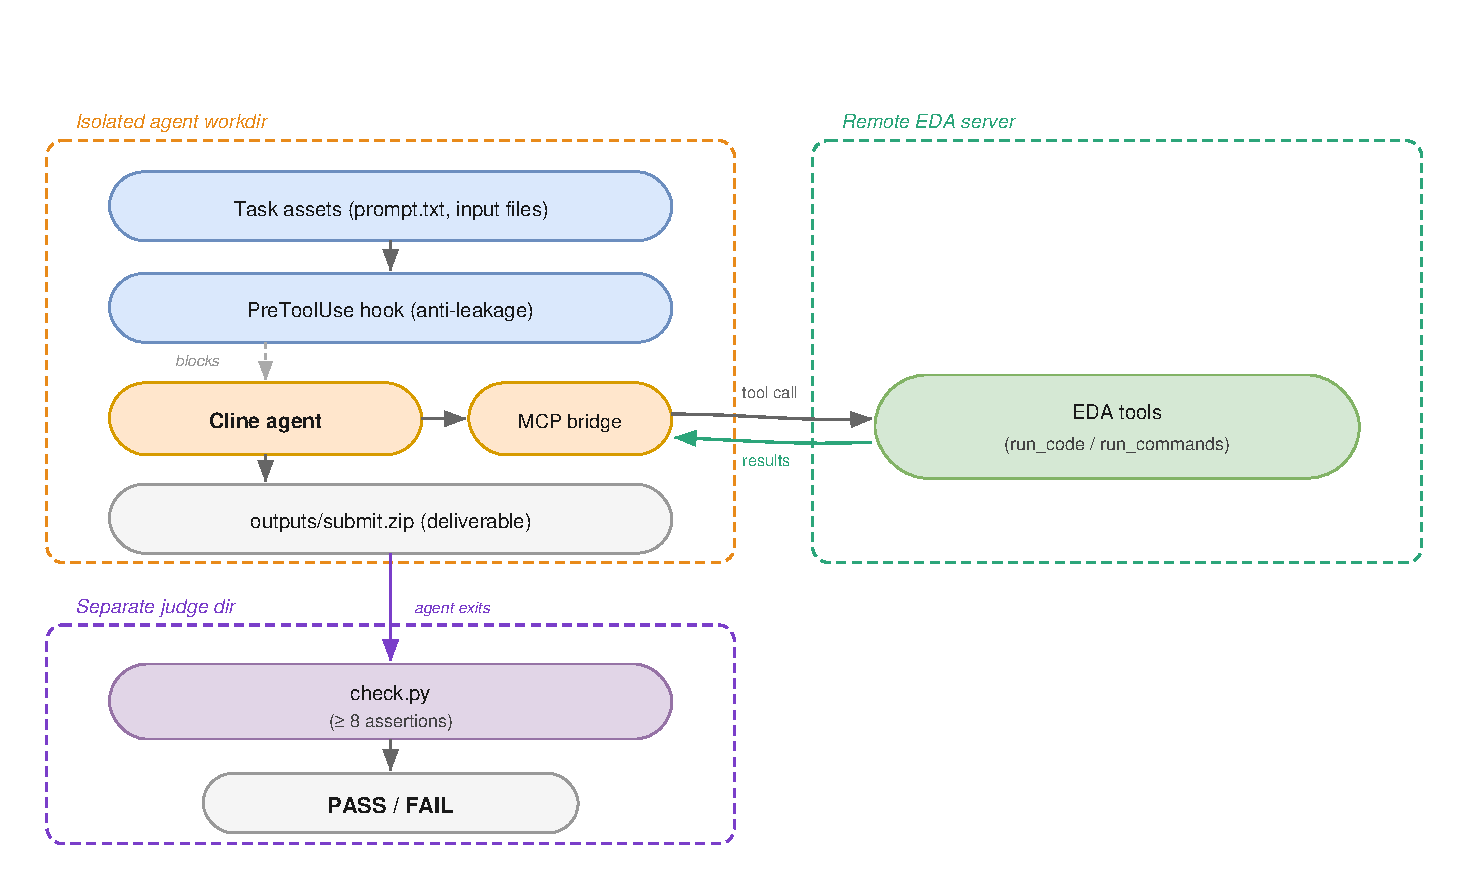
\includegraphics[width=\linewidth]{figures/pipeline.pdf}
\caption{Evaluation pipeline. The agent operates in an isolated workdir with EDA tools accessible only via MCP. The judge runs in a separate directory after agent completion.}
% \caption{评测流水线。智能体在隔离工作目录中运行，EDA 工具仅能通过 MCP 访问。判分器在智能体完成后于独立目录中运行。}
\label{fig:pipeline}
\end{figure}

\subsection{Anti-Leakage Protocol}
\label{sec:anti-leakage}
% \subsection{防泄题协议}

Answer leakage---the agent reading the answer key directly---is the single largest threat to benchmark validity. We enforce isolation through three layers:
% 答案泄露——智能体直接读取答案——是基准有效性最大的威胁。我们通过三层隔离来防范：

\begin{itemize}
    \item \textbf{Filesystem isolation}: The workdir contains only task assets and \texttt{prompt.txt}. The reference \texttt{check.py} and \texttt{reference/} directory are never copied into the workdir.
    % \textbf{文件系统隔离}：工作目录只含任务附件和 \texttt{prompt.txt}。参考 \texttt{check.py} 与 \texttt{reference/} 目录从不拷入工作目录。
    \item \textbf{PreToolUse hook}: A shell hook intercepts every tool call and blocks access to paths matching \texttt{check.py}, \texttt{\_check.py}, \texttt{reference/}, \texttt{hidden/}, and any file outside the workdir. Blocked calls return ``ACCESS RESTRICTED'' to the agent.
    % \textbf{PreToolUse 钩子}：一个 shell 钩子拦截每次工具调用，阻止访问匹配 \texttt{check.py}、\texttt{\_check.py}、\texttt{reference/}、\texttt{hidden/} 及工作目录之外的任何文件。被拦截的调用向智能体返回"ACCESS RESTRICTED"。
    \item \textbf{Scope management}: The hook scope is set to the evaluation workdir root, ensuring concurrent evaluations don't cross-access.
    % \textbf{作用域管理}：钩子作用域设为评测工作目录根，确保并发评测不会互相越权访问。
\end{itemize}

We verify isolation by counting \texttt{ACCESS RESTRICTED} events in each session log (\texttt{hook\_blocks} field in \texttt{status.jsonl}).
% 我们通过统计每份会话日志中的 \texttt{ACCESS RESTRICTED} 事件（\texttt{status.jsonl} 的 \texttt{hook\_blocks} 字段）来验证隔离是否生效。

\subsection{EDA Server Bridge}
\label{sec:eda-bridge}
% \subsection{EDA 服务器网桥}

The EDA server (10.129.32.75) provides:
% EDA 服务器（10.129.32.75）提供：
\begin{itemize}
    \item \textbf{Session management}: \texttt{open\_session} creates an isolated workdir; \texttt{close\_session} archives and removes it.
    % \textbf{会话管理}：\texttt{open\_session} 创建隔离工作目录；\texttt{close\_session} 归档并删除它。
    \item \textbf{Command execution}: \texttt{run\_commands} runs shell/EDA commands in the session workdir (bash -lc).
    % \textbf{命令执行}：\texttt{run\_commands} 在会话工作目录中运行 shell/EDA 命令（bash -lc）。
    \item \textbf{Code execution}: \texttt{run\_code} executes pyAether/SKILL/Tcl code in the appropriate EDA interpreter.
    % \textbf{代码执行}：\texttt{run\_code} 在对应的 EDA 解释器中执行 pyAether/SKILL/Tcl 代码。
    \item \textbf{File I/O}: \texttt{read\_file}/\texttt{write\_file} for EDA-side file access.
    % \textbf{文件读写}：\texttt{read\_file}/\texttt{write\_file} 用于 EDA 侧文件访问。
\end{itemize}

The agent must call \texttt{open\_session} first to obtain a workdir, then pass it to all subsequent calls. This mirrors real EDA workflow patterns where engineers open a design session before running tools.
% 智能体必须先调用 \texttt{open\_session} 取得工作目录，再将其传入所有后续调用。这映照了真实的 EDA 工作流习惯——工程师在运行工具前先打开一个设计会话。

\section{Experiments}
\label{sec:experiments}

\subsection{Experimental Setup}
\label{sec:exp-setup}
% \subsection{实验设置}

\textbf{Research questions.}
% \textbf{研究问题。}
\begin{itemize}
    \item \textbf{RQ1 (orchestration ceiling).} How well do frontier LLM agents perform on multi-step EDA design-flow orchestration, and how does this compare to single-script EDA benchmarks?
    % \textbf{RQ1（编排天花板）}：前沿 LLM 智能体在多步 EDA 设计流编排上表现如何？与单脚本 EDA 基准相比如何？
    \item \textbf{RQ2 (domain gap).} Which EDA domains are hardest for agents, and what drives the gap?
    % \textbf{RQ2（领域差距）}：哪些 EDA 领域对智能体最难？差距由什么驱动？
    \item \textbf{RQ3 (model scaling).} Does scaling the backbone close the orchestration gap, or is it bounded by tool-chain grounding?
    % \textbf{RQ3（模型扩展）}：扩大骨干模型能否弥合编排差距？还是受工具链接地能力约束？
\end{itemize}

\textbf{Benchmark.} \bench{} with \Ntasks{} curated cases across 13 domains (Section~\ref{sec:benchmark}); the results below use the frozen \Neval{}-run evaluation snapshot. We report Pass@1 (one trace per run, 2400s timeout, \texttt{thinking=low}).
% \textbf{基准。} \bench{}，含 \Ntasks{} 个已整理案例、覆盖 13 个领域（第~\ref{sec:benchmark}~节）；下方结果使用冻结的 \Neval{}-run 评测快照。我们报告 Pass@1（每 run 一次轨迹，超时 2400 秒，\texttt{thinking=low}）。

\textbf{Model.} A single frontier backbone, DeepSeek-V4-Pro, accessed via an OpenAI-compatible agi-gateway. A multi-backbone sweep (GLM-5.2, Kimi-K2.6, DeepSeek-V4-Flash, Doubao-Seed-2.0-Pro) is configured but not yet run to completion, so this paper reports a \emph{single-backbone} evaluation; RQ3 is therefore discussed as an open question in Section~\ref{sec:model-scaling}.
% \textbf{模型。} 单一前沿骨干模型 DeepSeek-V4-Pro，经 OpenAI 兼容的 agi-gateway 访问。多骨干扫描（GLM-5.2、Kimi-K2.6、DeepSeek-V4-Flash、Doubao-Seed-2.0-Pro）已配置但尚未跑完，故本文给出的是\emph{单骨干}评测；因此 RQ3 在第~\ref{sec:model-scaling}~节作为开放问题讨论。

\textbf{Harness.} Cline v3.0.51 with \texttt{PreToolUse} anti-leakage hook (Section~\ref{sec:anti-leakage}). Each task runs in a fresh workdir with EDA tools accessible via MCP bridge.
% \textbf{框架。} Cline v3.0.51，配 \texttt{PreToolUse} 防泄题钩子（第~\ref{sec:anti-leakage}~节）。每个任务在全新工作目录中运行，通过 MCP 网桥访问 EDA 工具。

\subsection{Main Results}
\label{sec:main-results}
% \subsection{主要结果}

\begin{table}[ht]
\centering
\caption{Main results on \bench: Pass@1 (\%) by domain, frozen 696-run evaluation (2026-11-09). Pass\% = PASS/(PASS+FAIL); ERROR (harness/tool infrastructure) and ABSENT (task assets unavailable) are reported but excluded from the denominator.}
% \caption{\bench{} 主要结果：各领域 Pass@1 (\%)，冻结的 696-run 评测（2026-11-09）。Pass\% = PASS/(PASS+FAIL)；ERROR（框架/工具基础设施）与 ABSENT（任务资产缺失）如实列出但不计入分母。}
% 注：完整配置 DeepSeek-V4-Pro / Cline v3.0.51 / thinking=low / 8 workers / 超时 2400s。
\label{tab:main-results}
\scriptsize
\setlength{\tabcolsep}{3pt}
\begin{tabular}{@{}lcccccc@{}}
\toprule
\textbf{Domain} & \textbf{PASS} & \textbf{FAIL} & \textbf{ERROR} & \textbf{ABSENT} & \textbf{Total} & \textbf{Pass\%} \\
\midrule
pnr\_signoff       & 5 & 19 & 0 & 1 & 25 & 20.8 \\
characterization   & 5 & 21 & 2 & 0 & 28 & 19.2 \\
eda\_other         & 6 & 27 & 4 & 1 & 38 & 18.2 \\
pg\_layout         & 4 & 24 & 0 & 0 & 28 & 14.3 \\
schematic\_netlist & 13 & 100 & 18 & 0 & 131 & 11.5 \\
digital            & 5 & 40 & 6 & 0 & 51 & 11.1 \\
layout\_virtuoso   & 4 & 35 & 0 & 1 & 40 & 10.3 \\
analog\_context    & 4 & 39 & 12 & 0 & 55 & 9.3 \\
verification       & 3 & 30 & 5 & 0 & 38 & 9.1 \\
spice\_sim         & 8 & 87 & 7 & 2 & 104 & 8.4 \\
waveform           & 2 & 37 & 8 & 0 & 47 & 5.1 \\
physical\_verify   & 2 & 66 & 4 & 1 & 73 & 2.9 \\
layout\_aether     & 1 & 33 & 4 & 0 & 38 & 2.9 \\
\midrule
\textbf{Overall}   & \textbf{62} & \textbf{558} & \textbf{70} & \textbf{6} & \textbf{696} & \textbf{10.0} \\
\bottomrule
\end{tabular}
\end{table}
% 逐行核验（PASS+FAIL+ERROR+ABSENT == Total，列合计 62/558/70/6/696，Pass% = 100*PASS/(PASS+FAIL) 四舍五入到 0.1）：
% 已用 scripts/audit 表校验脚本在本地跑过，13 行全对；校验脚本见
% doc/ZhuLong_DAC2027/benchmark/designflow/eval_triage/table_check.py

Table~\ref{tab:main-results} shows Pass@1 by domain on the frozen evaluation of \Neval{} runs across all 13 EDA domains (DeepSeek-V4-Pro, Cline v3.0.51, \texttt{thinking=low}). The overall Pass@1 of \textbf{10.0\%} (62/620 decided runs)\footnote{All pass rates use the \emph{decided} denominator (PASS$+$FAIL $=620$). The full batch comprises \Neval{} runs: 62 PASS, 558 FAIL, 70 ERROR (harness/tool infrastructure, undecided) and 6 ABSENT (task assets unavailable). Counting ABSENT as failure gives $62/626=9.9\%$ (95\% Wilson CI $[7.8,12.5]$); counting ERROR as failure gives $62/696=8.9\%$ ($[7.0,11.3]$). Our headline figure is $62/620=10.0\%$ (95\% Wilson CI $[7.9,12.6]$); the three estimators lie within $1.1$\,pp of each other and their confidence intervals overlap, so no conclusion below depends on the choice of denominator.} is dramatically lower than the 76.5\% reported on EDA-Scripting-Bench~\cite{zhu2026edascript} for single-script tasks, confirming that \emph{multi-step flow orchestration is qualitatively harder} than isolated code generation (RQ1).
% 表~\ref{tab:main-results} 展示了覆盖全部 13 个 EDA 领域、共 \Neval{} 个 run 的冻结评测的各领域 Pass@1（DeepSeek-V4-Pro、Cline v3.0.51、\texttt{thinking=low}）。总体 Pass@1 为 \textbf{10.0\%}（62/620 已判定 run），远低于 EDA-Scripting-Bench 上单脚本任务报告的 76.5\%，印证了"多步流程编排比孤立的代码生成在本质上更难"(RQ1)。
% 脚注口径：所有通过率使用"已判定分母"(PASS+FAIL=620)：62/620 = 10.0%（Wilson 95% CI [7.9, 12.6]）。
% 全批次 696 = 62 PASS + 558 FAIL + 70 ERROR（框架/工具基础设施故障，未判定）+ 6 ABSENT（任务资产缺失）。
% 若把 6 个 ABSENT 计为失败：62/626 = 9.9%（CI [7.8, 12.5]）；若把 70 个 ERROR 计为失败：62/696 = 8.9%（CI [7.0, 11.3]）。
% 三个估计量相差 ≤1.1pp 且置信区间重叠，故本文任何结论都不依赖分母选择。CI 由 eval_triage/ci_wilson.py 计算。

\subsection{Domain Gap (RQ2)}
\label{sec:domain-gap}
% \subsection{领域差距 (RQ2)}

The domain gap is large and consistent with the grounding-depth hypothesis: standardized-flow domains whose deliverable is largely a script or tcl template---\textbf{pnr\_signoff} (20.8\%), \textbf{characterization} (19.2\%), \textbf{eda\_other} (18.2\%)---pass at roughly twice the overall rate, while domains that require deep live-tool interaction---\textbf{physical\_verify} (2.9\%, DRC/LVS rule decks + run inspection) and \textbf{layout\_aether} (2.9\%, SKILL/GUI-driven layout editing)---sit at the bottom. The $7.1\times$ point-estimate ratio between the best and worst domain should be read as descriptive rather than established: with 24 decided runs in pnr\_signoff (Wilson 95\% CI $[9.2,40.5]$) and 68 in physical\_verify ($[0.8,10.1]$), the intervals overlap, and a single flipped run moves pnr\_signoff from 20.8\% to 24.0\%. What is robust is the \emph{ordering}: every standardized-flow domain sits above the overall rate and both deep-grounding domains sit at the bottom. The difference is not explained by task difficulty alone---all domains require EDA domain knowledge. The difference lies in \emph{tool-chain grounding depth}:
% 领域差距较大，且与接地深度假设一致：交付件主要为脚本或 tcl 模板的标准化流程领域——\textbf{pnr\_signoff}（20.8\%）、\textbf{characterization}（19.2\%）、\textbf{eda\_other}（18.2\%）——通过率约为整体的两倍，而需要深度实时工具交互的领域——\textbf{physical\_verify}（2.9\%，DRC/LVS 规则卡 + 运行检视）与 \textbf{layout\_aether}（2.9\%，SKILL/GUI 驱动的版图编辑）——垫底。最好/最差领域的 7.1 倍点估计应按描述性读，而非"已确立"：pnr\_signoff 仅 24 个已判定 run（Wilson 95\% CI [9.2,40.5]），physical\_verify 68 个（CI [0.8,10.1]），区间重叠；单个 PASS 翻转就能把 pnr\_signoff 从 20.8\% 推到 24.0\%。稳健的是\emph{排序}：所有标准化流程领域都高于总体，两个深度接地领域都在底部。该差距无法仅用任务难度解释——所有领域都需要 EDA 领域知识。差异在于"工具链接地深度"：

\begin{itemize}
    \item Standardized-flow tasks (pnr\_signoff, characterization, eda\_other) are largely \emph{text-in, script-out}: the agent reads a spec, writes a PrimeTime/Innovus tcl flow or a characterization script, and the deliverable follows a relatively fixed template. The agent can produce much of it from prior knowledge with only light tool interaction.
    % 标准化流程任务（pnr\_signoff、characterization、eda\_other）大体是"文本进、脚本出"：智能体读取规格、编写 PrimeTime/Innovus tcl 流程或表征脚本，交付件遵循相对固定的模板。智能体可凭先验知识产出大部分内容，仅需少量工具交互。
    \item Physical-verification and layout-editing tasks require \emph{deep tool grounding}: the agent must drive Calibre/PVS or Aether SKILL, inspect DRC/LVS results, interpret tool-specific error messages, and iterate on the rule deck or layout until the run is clean. Each iteration requires interpreting domain-specific tool outputs that the LLM cannot produce from prior knowledge alone.
    % 物理验证与版图编辑任务需要"深度工具接地"：智能体必须驱动 Calibre/PVS 或 Aether SKILL、检视 DRC/LVS 结果、解读工具专属错误信息，并迭代规则卡或版图直至运行干净。每一次迭代都需要解读领域专属的工具输出，而这是 LLM 无法仅凭先验知识生成的。
\end{itemize}

\subsection{Model Scaling (RQ3)}
\label{sec:model-scaling}
% \subsection{模型扩展 (RQ3)}

We report a single-backbone evaluation, so we cannot answer RQ3 empirically and
deliberately do not claim to. The relevant external evidence is that on
EDA-Scripting-Bench~\cite{zhu2026edascript} moving from the weakest to the
strongest backbone yields 23.3\,pp, while increasing observation fidelity of the
harness yields 56.8\,pp---i.e.\ on \emph{single-script} tasks the grounding axis
dominates the backbone axis. Whether the same holds when the task itself is a
multi-step flow is an open question: the 10.0\% vs.\ 76.5\% gap is a
\emph{cross-benchmark} comparison, confounded by task type, and therefore cannot
by itself show that model scaling is insufficient. We state this as a hypothesis
to be tested by the multi-backbone sweep (Section~\ref{sec:per-model}) rather than
as a finding, and we flag it again among the threats to validity
(Section~\ref{sec:threats}).
% 本文只做了单骨干评测，因此无法实证回答 RQ3，也刻意不作此断言。相关外部证据是：在
% EDA-Scripting-Bench 上，骨干从最弱换到最强带来 23.3pp，而提高框架的观测保真度带来 56.8pp
% ——即在"单脚本"任务上接地轴压过骨干轴。这一规律在多步流程任务上是否成立是开放问题：
% 10.0% vs 76.5% 是"跨基准"比较，被任务类型混淆，本身不能证明模型扩展不够。我们把它作为
% 待多骨干扫描检验的假设，而不是发现；并在有效性威胁一节再次标注。

\section{Analysis}
\label{sec:analysis}

% 注：原 "Analysis and Discussion" 拆分——本节聚焦实证分析（failure taxonomy / grounding depth / distribution），
% "Discussion" 内容移到 §\ref{sec:conclusion} 的 Conclusion 部分。
% 注：原"分析与讨论"已拆分——本节聚焦实证分析（失败分类法 / 接地深度 / 分布），
% "讨论"内容移到第~\ref{sec:conclusion}~节的结论部分。

\subsection{Failure Taxonomy}
\label{sec:failure-taxonomy}
% \subsection{失败分类法}

\textbf{Taxonomy protocol.} We define three mutually exclusive failure modes over the \Neval{} runs: (i) \emph{no-output / aborted}, where the run ends in ERROR (70 runs) or yields no \texttt{submit.zip} (among them the 6 ABSENT runs whose assets were unavailable); (ii) \emph{semantic / partial failure}, where a deliverable exists but at least one reference assertion fails (a subset of the 558 FAIL runs); and (iii) \emph{contract / format failure}, where the content is plausible but file-layout or naming assertions fail. The batch records only the terminal status per run, not which assertion failed first, so the run-level outcome counts we can state with certainty are PASS 62 / FAIL 558 / ERROR 70 / ABSENT 6 of \Neval{}. A systematic per-run labelling pass (\texttt{eval\_triage/05\_batch\_triage.py}, which derives each class from machine-checkable evidence and reports an explicit UNKNOWN share, never folding unclassified runs into another bucket) applied to the per-run judge logs of this batch yields the following measured split over the \Neval{} runs: (i) no-output / aborted = 146/696 = 21.0\% (the 70 ERROR runs plus the 6 ABSENT runs by terminal status, plus 70 FAIL runs that produced no \texttt{submit.zip}); (ii) semantic / partial failure = 437/696 = 62.8\% (132 \emph{ASSERT\_RUNTIME} runs where the candidate script crashed or exited non-zero, and 305 \emph{ASSERT\_SEMANTIC} runs where a reference assertion failed); (iii) contract / format failure = 2/696 = 0.3\%. The residual UNKNOWN is 49/696 = 7.0\%---FAIL runs that did produce a deliverable but whose released judge log exposes no machine-checkable failed-condition label (15 held-out-input setup gaps on the judge side, 12 check return-contract gaps, and 22 structured multi-condition results whose failing branch is not labelled in the truncated 300-char log). The tool's class-level UNKNOWN share is 119/696 = 17.1\%, which additionally includes the 70 ERROR-status runs (already counted in (i) by terminal status) whose abort reason---predominantly a missing per-case asset directory (59/70)---carries no timeout/infrastructure signature. The per-domain category matrix is reported in Appendix~\ref{sec:failure-by-domain}.
% \textbf{分类协议。} 我们在 \Neval{} 个 run 上定义三类互斥的失败模式：(i) 无输出/中止——
% run 以 ERROR 终止（70 个），或未产出 submit.zip（其中含 6 个资产缺失的 ABSENT）；
% (ii) 语义/部分失败——有交付件但至少一条参考断言不通过（558 个 FAIL 的子集）；
% (iii) 契约/格式失败——内容合理但文件结构或命名断言不通过。批次只记录每个 run 的终态，
% 故能确证的 run 级计数为 PASS 62 / FAIL 558 / ERROR 70 / ABSENT 6（共 \Neval{}）。用逐 run
% 归因工具（eval_triage/05_batch_triage.py，每类均由机器可核验证据推导并显式报告 UNKNOWN，
% 不把未分类 run 并入别桶）对本批逐 run 判分日志归因，得到实测占比：(i)=146/696=21.0%（70 ERROR
% +6 ABSENT 按终态 +70 个未产出 submit.zip 的 FAIL）；(ii)=437/696=62.8%（132 ASSERT_RUNTIME
% 候选脚本崩溃/非零退出 +305 ASSERT_SEMANTIC 参考断言失败）；(iii)=2/696=0.3%。残余 UNKNOWN=
% 49/696=7.0%——产出交付件但判分日志无可核验失败条件标签的 FAIL（15 个判分侧 hidden-B 输入缺失
% +12 个 check 返回契约缺口 +22 个多条件结构化结果其失败分支未在 300 字符截断日志中标注）。
% 工具类级 UNKNOWN=119/696=17.1%，另含 70 个 ERROR 终态 run（已按终态计入 (i)），其中止原因
% 多为单 case 资产目录缺失（59/70），无 timeout/infra 签名。逐域类别矩阵见附录~\ref{sec:failure-by-domain}。

\textbf{(1) No-output / aborted failures.} The agent produces no deliverable (\texttt{submit.zip} absent) or the run terminates in ERROR before judging. These are predominantly \emph{grounding failures}: the agent cannot determine which EDA tools to call, or calls them incorrectly, and gives up without producing any files. Among the failed traces we inspected, aborted and errored runs were concentrated in the deepest-grounding domains---physical\_verify and layout\_aether, where driving Calibre/PVS or Aether SKILL to a clean run is the binding obstacle.
% \textbf{(1) 无输出/中止失败}：智能体未产出交付件（submit.zip 缺失）或运行在判分前以 ERROR 终止。
% 这些主要是"接地失败"：弄不清该调用哪些 EDA 工具、或调用方式错误，最终放弃且未产出文件。
% 在我们检视过的失败轨迹中，中止与报错集中于接地最深的领域——physical_verify 与 layout_aether。

\textbf{(2) Semantic / partial failures.} The agent produces a deliverable but it fails $\geq 1$ assertion. These are \emph{semantic failures}: the deliverable is syntactically plausible but semantically incorrect---e.g., a SPICE deck that runs but produces wrong measurements, or a DRC script that checks the wrong rules. They dominate the medium-grounding domains (spice\_sim, verification, schematic\_netlist).
% \textbf{(2) 语义/部分失败}：智能体产出了交付件，但至少 1 条断言未通过。这些是"语义失败"：
% 交付件在语法上看似合理但语义不正确——例如 SPICE 卡能跑但测量值错，或 DRC 脚本查错规则。
% 它们在中度接地领域（spice_sim、verification、schematic_netlist）占主导。

\textbf{(3) Contract / format failures.} The deliverable is correct in content but fails format assertions (wrong file structure, missing files, wrong naming). These are \emph{contract failures}: the agent misunderstood the deliverable specification.
% \textbf{(3) 契约/格式失败}：交付件内容正确但未通过格式断言（文件结构错、缺文件、命名错）。
% 这些是"契约失败"：智能体误解了交付件规范。

\subsection{Tool-Chain Grounding Depth}
\label{sec:grounding-depth}
% \subsection{工具链接地深度}

We define \emph{grounding depth} as the minimum number of live EDA tool calls needed to produce a correct deliverable. Depth is not measured; it is an annotation we assign per domain (a design choice, stated as such). Figure~\ref{fig:grounding-depth} plots Pass@1 per depth bin, with each bin's value the mean of its domains' Pass@1 in Table~\ref{tab:main-results}:
% 我们将"接地深度"定义为产出正确交付件所需的最少真实 EDA 工具调用次数。深度不是测量值，
% 而是我们按领域手工标注的量（属设计选择，如实声明）。图~\ref{fig:grounding-depth} 按深度分箱
% 画出 Pass@1，每箱的取值是其所属领域在表~\ref{tab:main-results} 中 Pass@1 的均值。

\begin{itemize}
    \item \textbf{Depth 1--2} (pnr\_signoff, characterization, eda\_other): 19.4\% (mean of 20.8, 19.2, 18.2). The deliverable is largely a script or tcl template the agent can produce from prior knowledge with only light tool interaction.
    % \textbf{深度 1--2}（pnr\_signoff、characterization、eda\_other）：19.4\%（20.8/19.2/18.2 的均值）。交付件主要是脚本或 tcl 模板，智能体可凭先验知识产出，仅需少量工具交互。
    \item \textbf{Depth 3} (pg\_layout): 14.3\%. \textbf{Depth 4} (schematic\_netlist, digital): 11.3\% (mean of 11.5, 11.1). The agent must call tools and inspect outputs, but the tool chain is relatively standardized; failures are mostly semantic (wrong measurements, wrong rules).
    % \textbf{深度 3}（pg\_layout）：14.3\%。\textbf{深度 4}（schematic\_netlist、digital）：11.3\%（11.5/11.1 的均值）。智能体必须调用工具并检视输出，但工具链相对标准化；失败多为语义失败。
    \item \textbf{Depth 5} (layout\_virtuoso, analog\_context, verification, spice\_sim): 9.3\% (mean of 10.3, 9.3, 9.1, 8.4).
    % \textbf{深度 5}（layout\_virtuoso、analog\_context、verification、spice\_sim）：9.3\%（10.3/9.3/9.1/8.4 的均值）。
    \item \textbf{Depth 6} (waveform): 5.1\%. \textbf{Depth 7+} (physical\_verify, layout\_aether): 2.9\% (both domains). The agent must drive Calibre/PVS or Aether SKILL, maintain state across many tool calls, interpret domain-specific outputs, and iterate---a capability that current LLMs lack.
    % \textbf{深度 6}（waveform）：5.1\%。\textbf{深度 7+}（physical\_verify、layout\_aether）：均 2.9\%。智能体必须驱动 Calibre/PVS 或 Aether SKILL、在多次工具调用间维护状态、解读领域专属输出并迭代——这是当前 LLM 所欠缺的能力。
\end{itemize}

\begin{figure}[ht]
\centering
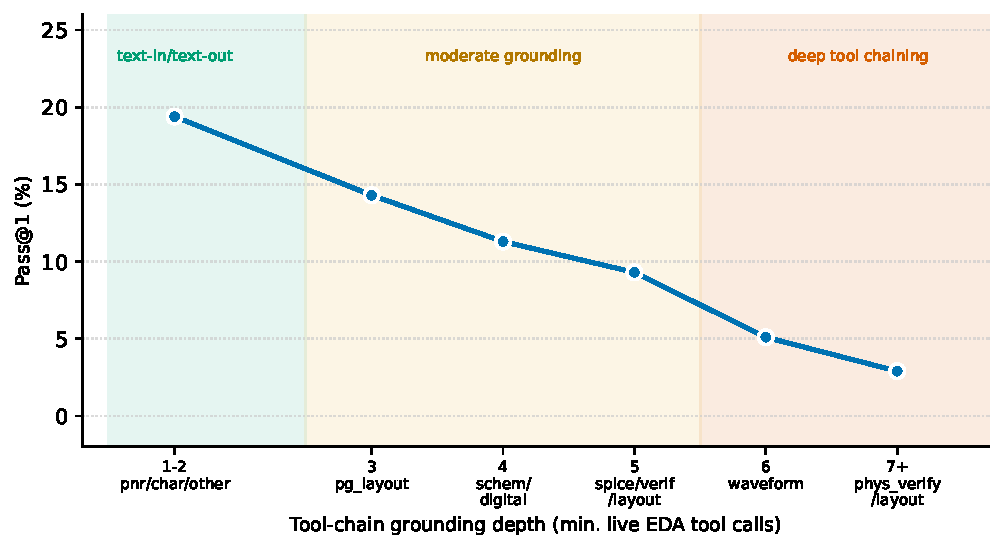
\includegraphics[width=\linewidth]{figures/grounding_depth.pdf}
\caption{Pass@1 by grounding-depth bin (domains grouped by our own annotation; the binning is a design choice, not a measured quantity). The ordering is descriptive: because depth is assigned by domain label, this figure does not by itself establish a causal or monotone relationship. Per-bin values are the means of the domains in Table~\ref{tab:main-results}.}
% \caption{按接地深度分箱的 Pass@1（分箱由我们手工标注，属设计选择而非测量量）。该排序是描述性的：
% 深度由领域标签指定，因此本图本身不能确立因果或严格单调关系。每箱取值见
% 表~\ref{tab:main-results} 中对应领域的均值。}
\label{fig:grounding-depth}
\end{figure}

\subsection{Trace Anatomy: A Pilot Study}
\label{sec:trace-anatomy}
% \subsection{轨迹解剖：试点研究}

To characterise \emph{how} runs behave rather than only whether they pass, we
instrumented 48 archived pilot runs (2026-11-03--11-06; 47 with a non-empty Cline
session log; 207\,MB, 1.21M events) and parsed every tool call, iteration and
termination record. This sample carries \emph{no judge verdict}---the pass/fail
labels live only in the batch runner---so the following are behavioural
statistics, not outcome attributions, and they are not extrapolated to the
\Neval{}-run evaluation.

\begin{itemize}
    \item \textbf{Effort.} The median run issues 26.5 tool calls (IQR 13.8--38.0,
    max 97) across 20.5 agent iterations (IQR 9.0--32.5), and runs for a median
    of 1{,}047\,s (IQR 552--1{,}495). Effort is therefore substantial but not
    unbounded: the deep-grounding tasks do not fail because the agent refuses to
    try.
    % \textbf{投入。} 中位 run 发出 26.5 次工具调用（IQR 13.8--38.0，最大 97），跨 20.5 轮
    % 迭代（IQR 9.0--32.5），中位耗时 1,047 秒（IQR 552--1,495）。投入可观但并非无界：
    % 深度接地任务失败并非因为智能体不肯尝试。
    \item \textbf{Tool mix.} Across 1{,}371 tool calls, 41.2\% go through the MCP
    bridge (\texttt{eda\_flow\_\_*}, \texttt{pyAether\_MCP\_server\_\_*}) and 58.8\%
    to built-in file/search/shell tools; \texttt{read\_files} alone is 28.8\% of
    all calls. The agent spends the plurality of its steps \emph{reading}, not
    driving EDA tools---consistent with an observation bottleneck rather than an
    action bottleneck.
    % \textbf{工具构成。} 1,371 次工具调用中 41.2\% 走 MCP 网桥，58.8\% 为内置文件/搜索/shell；
    % 单 read_files 占 28.8%。智能体的多数步骤用于\emph{读}而非驱动 EDA 工具——与"瓶颈在观测
    % 而非动作"一致。
    \item \textbf{Termination.} 27 runs end normally (\texttt{finishReason=completed}),
    6 terminate with an \texttt{error} event, 3 were aborted by a human, and 11
    archives are truncated mid-stream (5 of them cut at 1{,}794--1{,}799\,s, i.e.\
    within 6\,s of a 30-minute mark). Truncation inflates apparent "no-output"
    rates, which is why we report run-level status separately from trace-level
    termination.
    % \textbf{终止形态。} 27 个 run 正常结束，6 个以 error 事件终止，3 个被人为中止，
    % 11 份归档在流中被截断（其中 5 份截在 1,794--1,799 秒，距 30 分钟整点 <6 秒）。
    % 归档截断会抬高表面上的"无输出"比例——这也是我们把 run 级状态与轨迹级终止分开报告的原因。
    \item \textbf{Two harness artefacts.} One case shows the wrapper failing before
    the agent started (\texttt{o-approve: command not found}) while its
    \texttt{outputs/} directory still contained files, and one run logged 2{,}565\,s
    despite the nominal 2{,}400\,s timeout. Both are harness-side defects that the
    batch-level status alone would mis-attribute to the model; they motivate the
    per-run triage tool shipped with the benchmark.
    % \textbf{两个框架侧缺陷。} 一例显示 wrapper 在 agent 启动前就失败
    % （o-approve: command not found），但 outputs/ 里仍留有文件；另一例记录了 2,565 秒，
    % 超过名义上的 2,400 秒超时。二者都是框架侧缺陷——只看批次级状态会把它们错记为模型问题；
    % 这也是我们随基准发布逐 run 归因工具的原因。
\end{itemize}

\subsection{Distribution Analysis}
\label{sec:distribution}
% \subsection{分布分析}

\bench's domain distribution (Figure~\ref{fig:domain-distribution}) reflects real engineering practice, as discussed in Section~\ref{sec:domain-coverage}. This is a \emph{feature} of trace-based benchmark construction: the distribution reflects actual agent usage patterns, not synthetic task design.
% \bench{} 的领域分布（图~\ref{fig:domain-distribution}）反映了真实工程实践，如第~\ref{sec:domain-coverage}~节所述。这是基于轨迹构建基准的一个"特性"：分布反映真实的智能体使用模式，而非合成的任务设计。

\subsection{Threats to Validity}
\label{sec:threats}
% \subsection{有效性威胁}

\textbf{Domain imbalance.} Counting the \Neval{} evaluated runs, the top three domains hold 44.3\% and digital-front domains 12.8\%. This reflects real usage but may bias aggregate metrics toward analog-friendly capabilities.
% \textbf{领域失衡。} 按 \Neval{} 个已评测 run 计，前三个领域占 44.3\%，数字前端类领域占 12.8\%。这反映了真实使用情况，但可能使聚合指标偏向对模拟友好的能力。

\textbf{Single backbone.} All \Neval{} runs use one backbone (DeepSeek-V4-Pro). Claims about ``the best'' or about model scaling are therefore not supported by our own data; RQ3 is reported as an open question (Section~\ref{sec:model-scaling}).
% \textbf{单一骨干。} \Neval{} 个 run 全部使用同一骨干（DeepSeek-V4-Pro）。因此"最优模型"或"模型扩展"的论断不由我们自己的数据支撑；RQ3 作为开放问题报告。

\textbf{Frozen snapshot.} Results are tied to the 2026-11-09 snapshot of \Neval{} runs over the Full set, which has since grown to \Ntasks{} cases. Adding cases changes the domain mix and the achievable score; comparisons across snapshots are not valid unless the snapshot is pinned. The Lite set (\LiteSet{} tasks, Appendix) is fixed to support reproducible daily evaluation.
% \textbf{冻结快照。} 结果绑定在 2026-11-09 的 \Neval{}-run 快照上（基于 Full 集），而 Full 集已增长至 \Ntasks{} 个案例。
% 新增案例会改变领域构成与可达分数；除非固定快照，跨快照比较无效。Lite 集（\LiteSet{} 个任务，见附录）已固定，以支持可复现的日常评测。

\textbf{Trace sample bias.} The behavioural statistics in Section~\ref{sec:trace-anatomy} come from 47 archived pilot logs, not from the \Neval{}-run batch: archived traces are those that survived local retention, and 11 of them are truncated. They describe mechanics (effort, tool mix, termination), not pass rates.
% \textbf{轨迹样本偏差。} 第~\ref{sec:trace-anatomy}~节的行为学统计来自 47 份归档 pilot 日志，而非 \Neval{}-run 批次：
% 能归档的是本地留存下来的轨迹，且其中 11 份被截断。它们描述机制（投入、工具构成、终止形态），不描述通过率。

\textbf{Single tool ecosystem.} All tasks use commercial EDA tools (Empyrean Aether, Cadence, Synopsys) accessible via a single EDA server. Generalization to open-source EDA (Yosys, OpenROAD, Magic) is not evaluated.
% \textbf{单一工具生态。} 所有任务使用商业 EDA 工具（华大九天 Aether、Cadence、Synopsys），通过单一 EDA 服务器访问。对开源 EDA（Yosys、OpenROAD、Magic）的泛化能力未作评估。

\textbf{Single agent harness.} We evaluate only Cline; other agent frameworks (SWE-agent, OpenHands, AutoGPT) may perform differently. However, the anti-leakage protocol and MCP bridge are agent-agnostic.
% \textbf{单一智能体框架。} 我们只评测了 Cline；其他智能体框架（SWE-agent、OpenHands、AutoGPT）可能表现不同。但防泄题协议与 MCP 网桥是与具体智能体无关的。

\textbf{Trace provenance.} Tasks are derived from real user sessions, which may contain company-specific conventions, PDK-specific constraints, or tool-version-specific behaviors that limit generalizability.
% \textbf{轨迹来源。} 任务源于真实用户会话，可能包含公司专属约定、PDK 专属约束或工具版本专属行为，从而限制泛化性。

\section{Related Work}
\label{sec:related}

\subsection{LLM Benchmarks for EDA and Hardware Design}
% \subsection{面向 EDA 与硬件设计的 LLM 基准}

\textbf{RTL code generation.} RTLLM~\cite{lu2024rtllm} introduced 30 (later 50) digital designs with natural-language specifications, testbenches, and reference RTL, evaluating syntax correctness, functional accuracy, and PPA quality. VerilogEval~\cite{liu2023verilogeval} extended this to 100+ Verilog tasks from diverse sources. Both evaluate \emph{single-module} generation---one function, one testbench---without tool interaction or multi-step orchestration. \bench{} differs fundamentally: each task requires the agent to call live EDA tools, inspect outputs, and produce a multi-file deliverable across multiple steps.
% \textbf{RTL 代码生成。} RTLLM 引入了 30 个（后扩至 50 个）数字设计，附带自然语言规格、测试台和参考 RTL，评估语法正确性、功能准确性和 PPA 质量。VerilogEval 将此扩展到来自多种来源的 100 多个 Verilog 任务。两者都评估"单模块"生成——一个函数、一个测试台——无工具交互、无多步编排。\bench{} 有根本不同：每个任务要求智能体调用真实 EDA 工具、检视输出、并跨多步产出多文件交付件。

\textbf{Flow repair.} FlowFixer-EDA~\cite{dong2026flowfixer} and EDA-FlowBench evaluate diagnosing and repairing failures in open-source RTL-to-GDS flows (Yosys, OpenROAD), with 200 tasks covering multiple error categories. While closer to real workflows, these benchmarks operate on \emph{open-source tools only} and evaluate \emph{repair} (fixing a broken run) rather than \emph{orchestration} (building a deliverable from scratch). \bench{} uses commercial EDA tools (Empyrean Aether, Cadence Virtuoso, Synopsys tools) and evaluates end-to-end deliverable production.
% \textbf{流程修复。} FlowFixer-EDA 和 EDA-FlowBench 评估在开源 RTL-to-GDS 流程（Yosys、OpenROAD）中诊断并修复失败，含 200 个任务覆盖多种错误类别。虽然更接近真实工作流，但这些基准仅操作"开源工具"，且评估的是"修复"（修复一次失败运行）而非"编排"（从零构建交付件）。\bench{} 使用商业 EDA 工具（华大九天 Aether、Cadence Virtuoso、Synopsys 工具），评估端到端的交付件生产。

\textbf{EDA scripting.} EDA-Scripting-Bench~\cite{zhu2026edascript} evaluates LLM agents on PyAether, SKILL, and Tcl scripting across 449 tasks with execution-based scoring. While sharing the execution-grounded philosophy, it evaluates \emph{single-script} generation (one function per task), not multi-step flow orchestration with deliverable packaging. \bench{} extends this to the \mode{} paradigm where the agent must produce a complete deliverable package.
% \textbf{EDA 脚本。} EDA-Scripting-Bench 在 pyAether、SKILL 和 Tcl 脚本上评估 LLM 智能体，含 449 个任务，采用执行式判分。虽然同样秉持"执行接地"的理念，但它评估的是"单脚本"生成（每任务一个函数），而非带交付件打包的多步流程编排。\bench{} 将此扩展到 \mode{} 范式，智能体须产出完整的交付件包。

\subsection{Agent Benchmarks in Software Engineering}
% \subsection{软件工程中的智能体基准}

SWE-bench~\cite{jimenez2024swebench} and its variants (SWE-bench Verified, SWE-bench Pro) evaluate whether AI agents can resolve real GitHub issues by editing codebases. The key insight---execution-based evaluation against a project's own test suite---inspires our design. However, SWE-bench operates on Python repositories with Docker-based evaluation, while \bench{} operates on EDA design flows with live commercial tool execution on a remote EDA server. The EDA setting introduces unique challenges: closed tools, non-redistributable data, and tool-chain grounding requirements that have no software-engineering analog.
% SWE-bench 及其变体（SWE-bench Verified、SWE-bench Pro）评估 AI 智能体能否通过编辑代码库来解决真实 GitHub issue。其核心洞见——基于项目自身测试套件进行执行式评估——启发了我们的设计。然而，SWE-bench 操作的是 Python 仓库并用 Docker 评估，而 \bench{} 操作的是 EDA 设计流，在远程 EDA 服务器上执行真实商业工具。EDA 场景引入了独特挑战：封闭工具、不可再分发数据，以及软件工程中不存在的工具链接地要求。

\subsection{Tool-Use and Execution-Grounded Agents}
% \subsection{工具使用与执行接地的智能体}

The MCP (Model Context Protocol)~\cite{lee2025autoeda} standardizes tool exposure to LLMs. Execution-grounded agents~\cite{zhu2026edascript, schick2024toolformer} close a generate--execute--refine loop by observing tool outputs. \bench{} evaluates agents in this paradigm: the agent must call EDA tools through an MCP bridge, read execution results (simulation logs, DRC reports, netlist extracts), and iteratively refine its deliverable. This is qualitatively harder than single-shot generation because the agent must maintain state across tool calls, interpret domain-specific outputs, and decide when the deliverable is complete.
% MCP（模型上下文协议）标准化了 LLM 的工具暴露方式。执行接地型智能体通过观测工具输出闭合"生成—执行—精炼"回路。\bench{} 在此范式下评估智能体：智能体必须通过 MCP 网桥调用 EDA 工具，读取执行结果（仿真日志、DRC 报告、网表抽取），并迭代精炼其交付件。这在本质上难于单次生成，因为智能体必须在多次工具调用间维护状态、解读领域专属输出，并判断交付件何时完成。
      % Related Work 放结果后（ML 惯例）
\section{Discussion and Conclusion}
\label{sec:conclusion}

% 注：原 §7 仅 Conclusion，现合并 Discussion 内容（SWE-bench 惯例：Discussion 单独成节或与 Conclusion 合并）。
% 注：原第 7 节仅含结论，现合并讨论内容（SWE-bench 惯例：讨论可单独成节或与结论合并）。

We presented \bench, the first benchmark for LLM agents on multi-step circuit design flow orchestration, built from real user interaction traces across 13 EDA domains (a living set of \Ntasks{} cases, evaluated here on a frozen \Neval{}-run snapshot). The evaluation yields a clear result: a single frontier backbone reaches 10.0\% Pass@1 on multi-step flow orchestration (62/620 decided runs), against 76.5\% reported for single-script EDA tasks. The ordering across domains---pnr\_signoff 20.8\% at the top, physical\_verify and layout\_aether at 2.9\% at the bottom---is stable even though the individual ratios are not: current agents do well when the deliverable is a script or template and poorly when deep live-tool interaction (DRC/LVS runs, GUI-driven layout editing) is required.
% 我们提出了 \bench，这是首个面向 LLM 智能体多步电路设计流编排的基准，构建于 13 个 EDA 领域的真实用户交互轨迹之上（活集 \Ntasks{} 例，本文在冻结的 \Neval{}-run 快照上评测）。
% 评测给出清晰结果：单一前沿骨干在多步流程编排上取得 10.0\% Pass@1（62/620 已判定 run），而单脚本 EDA 任务上报告为 76.5\%。
% 领域间排序——pnr_signoff 20.8\% 居首，physical_verify 与 layout_aether 均 2.9\% 垫底——稳健，但单个比值并不稳健：当交付件是脚本/模板时当前智能体表现尚可，需要深度实时工具交互（DRC/LVS 运行、GUI 版图编辑）时则失败。

\textbf{Implications.} The grounding-depth bottleneck suggests two research directions: (i) \emph{retrieval-augmented tool use}, where the agent retrieves tool documentation and prior execution traces to ground its tool calls, and (ii) \emph{execution-feedback loops}, where intermediate tool outputs are explicitly fed back as context. Neither is fully solved by scaling the backbone alone. Our benchmark provides a testbed for evaluating such interventions.
% \textbf{启示。} 接地深度瓶颈提示了两个研究方向：(i)"检索增强的工具使用"——智能体检索工具文档和历史执行轨迹来为自己的工具调用接地；(ii)"执行反馈回路"——把中间工具输出显式回填为上下文。两者都无法仅靠扩大骨干模型来解决。我们的基准为评估此类干预手段提供了测试床。

\textbf{Future work.}
% \textbf{未来工作。}
\begin{itemize}
    \item \textbf{Expand domain coverage}: supplement digital synthesis and verification tasks to balance the distribution.
    % \textbf{扩展领域覆盖}：补充数字综合与验证任务以均衡分布。
    \item \textbf{Multi-agent evaluation}: evaluate agent frameworks beyond Cline (SWE-agent, OpenHands).
    % \textbf{多智能体评测}：评估 Cline 之外的智能体框架（SWE-agent、OpenHands）。
    \item \textbf{Open-source EDA}: extend the benchmark to open-source tool chains (Yosys, OpenROAD, Magic) for reproducibility.
    % \textbf{开源 EDA}：将基准扩展到开源工具链（Yosys、OpenROAD、Magic）以提升可复现性。
    \item \textbf{Grounding interventions}: develop and evaluate techniques to improve tool-chain grounding (retrieval-augmented tool use, execution-feedback loops, tool-documentation pretraining).
    % \textbf{接地干预}：开发并评估改善工具链接地的技术（检索增强工具使用、执行反馈回路、工具文档预训练）。
\end{itemize}

\bench{} is built from proprietary user interaction traces that constitute company intellectual property and therefore cannot be publicly released in their original form. To balance reproducibility with these confidentiality constraints, we commit to releasing: (i) the evaluation harness (\texttt{run\_one.sh}, \texttt{run\_batch.sh}, anti-leakage hook, MCP bridge configuration) as open-source scripts; (ii) a \emph{sanitized task specification set} with prompts, reference assertions, and \texttt{check.py} judges for a representative subset of tasks whose underlying designs have been approved for external release; and (iii) a \emph{mock-EDA mode} enabling harness testing without commercial tool licenses. Full details of the release plan, the sanitization protocol, and the open-source-EDA extension roadmap are described in the Reproducibility Statement (Section~\ref{sec:reproducibility}).
% \bench{} 构建于构成公司知识产权的专有用户交互轨迹之上，因此无法以原始形式公开发布。为在可复现性与保密约束之间取得平衡，我们承诺发布：(i) 评测框架（\texttt{run\_one.sh}、\texttt{run\_batch.sh}、防泄题钩子、MCP 网桥配置）作为开源脚本；(ii) 一套\emph{脱敏任务规格集}，包含经批准可对外发布的代表性子集任务的提示词、参考断言和 \texttt{check.py} 判分器；以及 (iii) 一套\emph{mock-EDA 模式}，无需商业工具许可证即可测试框架。发布计划、脱敏协议和开源 EDA 扩展路线图的完整细节见可复现性声明（第~\ref{sec:reproducibility}~节）。


% ===== Ethics + Reproducibility（ICML 强制）=====
\section*{Ethics Statement}
\label{sec:ethics}

% ICML 强制要求。讨论数据来源伦理、潜在双重用途、隐私保护。

\textbf{Data provenance and consent.} \bench{} is derived from real user interaction traces of IC design engineers using the Cline coding agent on their workstations. The trace collection was conducted as part of routine infrastructure monitoring of an internal engineering environment, with the knowledge and consent of the engineering organization. No personally identifying information (PII) beyond usernames is retained; usernames are preserved for reproducibility and trace-back but are internal corporate identifiers, not public identities. All API keys, tokens, and passwords found in session logs are masked before task curation.

\textbf{Proprietary data and tools.} All tasks use commercial EDA tools (Empyrean Aether, Cadence Virtuoso, Synopsys) accessed through a licensed EDA server. The benchmark release includes task specifications, prompts, and reference assertions, but \emph{not} the proprietary tool licenses, PDK files, or design data. External users must provide their own EDA licenses to reproduce results. This limits reproducibility in open settings; we discuss this trade-off in Appendix~\ref{sec:repro-details} and propose an open-source-EDA extension as future work.

\textbf{Dual-use considerations.} The benchmark measures agent capability on EDA design flows. Improvements on \bench{} could accelerate chip design automation, with broad societal benefit (faster semiconductors, lower design cost). We do not foresee direct dual-use risks: the benchmark does not expose classified designs, does not target security-critical circuits, and the evaluated capability (writing EDA glue scripts) is a general engineering skill, not a weaponizable capability.

\textbf{Labor impact.} Benchmarks that measure automation of engineering tasks may be used to justify workforce reductions. We emphasize that \bench{} measures \emph{agent capability on flow orchestration}, which at 28\% Pass@1 is far below the threshold for autonomous replacement of engineers. The benchmark is intended to \emph{guide capability development}, not to evaluate individual engineers. We discourage using \bench{} results for personnel evaluation.

\textbf{Bias and representation.} The domain distribution reflects the usage patterns of one engineering organization, which may not represent the global EDA community. Analog/mixed-signal and physical-verification tasks are over-represented; digital-synthesis tasks are under-represented. Consumers of the benchmark should weight domain-specific results rather than aggregate scores alone.

\section*{Reproducibility Statement}
\label{sec:reproducibility}

% ICML 期望。说明代码/数据/模型/框架的可复现性。
% ICML 期望。说明代码/数据/模型/框架的可复现性。

\textbf{Confidentiality constraint.} The core asset of \bench---the real user interaction traces from which all \Ntasks{} tasks are derived---constitutes proprietary intellectual property of the IC design organization. These traces contain company-specific design data, PDK references, and engineer workflows that cannot be redistributed under the organization's data governance policy. We therefore adopt a \emph{tiered release strategy} that separates methodological reproducibility (which we fully support) from exact-data reproducibility (which is constrained), following the approach used by other industrial benchmarks built on confidential data~\cite{rao2026sap, sulthanpete2026nyris}.
% \textbf{保密约束。} \bench{} 的核心资产——所有 \Ntasks{} 个任务所源自的真实用户交互轨迹——构成 IC 设计组织的专有知识产权。这些轨迹包含公司专属设计数据、PDK 引用和工程师工作流，根据组织的数据治理政策不可再分发。因此我们采用\emph{分层发布策略}，将方法可复现性（我们完全支持）与精确数据可复现性（受约束）分离，这一做法与其他基于保密数据的工业基准一致。

\textbf{What we release.}
% \textbf{我们发布什么。}
\begin{itemize}
    \item \textbf{Evaluation harness (open-source).} The full \texttt{run\_one.sh} / \texttt{run\_batch.sh} harnesses, the \texttt{PreToolUse} anti-leakage hook, and the MCP bridge configuration are released as open-source scripts. The harness is agent-agnostic: any coding agent supporting MCP and shell hooks can be evaluated.
    % \textbf{评测框架（开源）。} 完整的 \texttt{run\_one.sh} / \texttt{run\_batch.sh} 框架、\texttt{PreToolUse} 防泄题钩子和 MCP 网桥配置作为开源脚本发布。框架与具体智能体无关：任何支持 MCP 和 shell 钩子的编程智能体均可被评测。
    \item \textbf{Sanitized task subset.} For tasks whose underlying designs have been approved for external release, we release the full task specification: prompt, input assets, reference assertions, \texttt{check.py} judge, and \texttt{test\_rationale}. This subset is sufficient to reproduce the evaluation protocol and compare new agents on a representative slice of \bench.
    % \textbf{脱敏任务子集。} 对于底座设计已获对外发布批准的任务，我们发布完整任务规格：提示词、输入附件、参考断言、\texttt{check.py} 判分器和 \texttt{test\_rationale}。该子集足以复现评测协议并在 \bench{} 的代表性切片上比较新智能体。
    \item \textbf{Task schema and construction protocol.} The JSONL schema, domain keyword filters, scan pipeline, and two-stage prefilter are fully documented (Appendix~\ref{sec:benchmark-details}), enabling other organizations with their own Cline traces to construct comparable benchmarks.
    % \textbf{任务模式与构建协议。} JSONL 模式、领域关键词过滤器、扫描流程和两级预筛器完整记录于附录~\ref{sec:benchmark-details}，使拥有自有 Cline 轨迹的其他组织能够构建可比基准。
    \item \textbf{Model configurations.} All evaluated models are accessed via an OpenAI-compatible API gateway. We release the exact \texttt{providers.json} configuration (with API keys masked), the thinking-budget setting (\texttt{thinking=low}), the per-task timeout (2400s), and the auto-approve policy.
    % \textbf{模型配置。} 所有受评模型通过 OpenAI 兼容 API 网关访问。我们发布精确的 \texttt{providers.json} 配置（API 密钥脱敏）、思考预算设置（\texttt{thinking=low}）、单任务超时（2400 秒）和自动批准策略。
    \item \textbf{Experimental logs.} Full \texttt{status.jsonl} records (verdict, duration, hook blocks, token usage per task) are released for all reported runs, enabling replication of every reported number on the released task subset.
    % \textbf{实验日志。} 所有报告运行的完整 \texttt{status.jsonl} 记录（每任务的判定、耗时、钩子拦截次数、token 用量）予发布，使发布任务子集上的每个报告数字可复现。
    \item \textbf{Mock-EDA mode.} A mock MCP bridge that returns canned tool outputs, enabling harness and hook testing without commercial EDA tool licenses.
    % \textbf{mock-EDA 模式。} 一个返回预设工具输出的 mock MCP 网桥，无需商业 EDA 工具许可证即可测试框架和钩子。
\end{itemize}

\textbf{What we cannot release.} The original user interaction traces, the unreleased task assets (RTL fragments, simulation logs, technology files, PDK data), and access to the specific commercial EDA tools (Empyrean Aether, Cadence Virtuoso, Synopsys) remain behind the organization's confidentiality boundary. Full reproduction of all \Ntasks{} tasks in their original form requires these assets and licenses, which we cannot provide to external parties.
% \textbf{我们不能发布什么。} 原始用户交互轨迹、未发布的任务附件（RTL 片段、仿真日志、工艺文件、PDK 数据）以及对特定商业 EDA 工具（华大九天 Aether、Cadence Virtuoso、Synopsys）的访问，仍留在组织的保密边界之内。以原始形式完整复现所有 \Ntasks{} 个任务需要这些资产和许可证，而我们无法向外部方提供。

\textbf{Mitigations and roadmap.} To address the reproducibility gap, we provide: (i) a \emph{judge-only mode} that runs \texttt{check.py} against any pre-packaged \texttt{submit.zip}, enabling verification of agent deliverables without live EDA tools; (ii) a roadmap for an open-source-EDA extension (Yosys, OpenROAD, Magic, ngspice) that maps each domain to an open-source equivalent (Appendix~\ref{sec:repro-details}); and (iii) a commitment to expand the sanitized task subset as more designs receive release approval.
% \textbf{缓解措施与路线图。} 为弥合可复现性差距，我们提供：(i) 一套"仅判分模式"，对任意预打包 \texttt{submit.zip} 运行 \texttt{check.py}，无需真实 EDA 工具即可验证智能体交付件；(ii) 一份开源 EDA 扩展路线图（Yosys、OpenROAD、Magic、ngspice），将每个领域映射到对应开源方案（附录~\ref{sec:repro-details}）；以及 (iii) 随更多设计获得发布批准而持续扩展脱敏任务子集的承诺。

\textbf{Statistical methodology.} We report Pass@1 (single trace per task). For aggregate scores, we report both raw counts and percentages. Confidence intervals are computed via Wilson score intervals at 95\% confidence.
% \textbf{统计方法。} 我们报告 Pass@1（每任务单次轨迹）。对于聚合分数，我们同时报告原始计数与百分比。置信区间采用 95\% 置信水平下的 Wilson 区间。


% ===== 参考文献 =====
\clearpage
\bibliographystyle{icml2026}
\bibliography{references}

% ===== 附录（不计入页数限制，放在 references 之后）=====
\newpage
\appendix
\section{Benchmark Details}
\label{sec:benchmark-details}

% 附录 A：benchmark 构建细节（参考 SWE-bench Appendix A "Benchmark Details"）

\subsection{Task Example}
\label{sec:task-example}

[TODO: 完整展示一个 task 的 prompt + assets + check.py + test\_rationale。建议选一个中等难度的 schematic\_netlist case，展示 design\_flow 契约的全貌。]

\subsection{Scan Pipeline Details}
\label{sec:scan-pipeline}

We systematically scanned 698 engineering workstations via SSH, searching session files for EDA-keyword matches. Sessions are ranked by match-count (mc)---the number of lines hitting any EDA keyword. The mc $\geq 30$ threshold yields 1{,}511 candidate sessions from 226 unique users.

\textbf{Two-stage prefilter.} A rule-based stage rejects sessions with $< 3$ EDA tool invocations or $> 50\%$ permission-denied lines. A 0.8B LLM classifier (Qwen3.5-0.8B-Q8\_0, CPU) performs a binary is\_design\_flow classification. End-to-end cost is $\sim$1.1s/call at 73 tok/s. On the full 1{,}369-session candidate pool, the prefilter rejects 0\%---confirming that mc $\geq 30$ sessions are almost universally genuine EDA work.

\subsection{Domain Keyword Filters}
\label{sec:keyword-filters}

Table~\ref{tab:keywords} lists the EDA keywords used for session scanning and shard assignment. Shard A uses an expanded keyword set (synthesis, synopsys, tcl, verilog, systemverilog, rtl, sdc, vivado, yosys, openroad) and a relaxed mc threshold ($\geq 15$) to capture digital-front tasks that use cline less intensively.

\begin{table}[ht]
\centering
\small
\caption{EDA keyword filters by shard.}
\label{tab:keywords}
\begin{tabular}{@{}lll@{}}
\toprule
\textbf{Shard} & \textbf{mc threshold} & \textbf{Keywords} \\
\midrule
A & $\geq 15$ & verdi, vcs, dc\_shell, innovus, primetime, synthesis, tcl, verilog, rtl \\
B & $\geq 30$ & hspice, finesim, siliconsmart, spectre, ngspice, simulator, spice \\
C & $\geq 30$ & calibre, virtuoso, aether, ipcustom, layout, lvs, drc \\
D & $\geq 30$ & waveview, cosmos, skill, netlist, spiros, spectrum, analog, schematic \\
\bottomrule
\end{tabular}
\end{table}

\subsection{Full Domain Distribution}
\label{sec:full-distribution}

[TODO: 完整 863 cases 的 domain 分布表 + 用户/主机分布。当前数据：A:176 B:200 C:260 D:249 = 863 cases, 226 去重用户, 13 domain。]

\subsection{Task Schema Specification}
\label{sec:task-schema-spec}

Each task is a JSONL record with the following fields:
\begin{itemize}
    \item \texttt{id}: unique task identifier (shard-prefixed, e.g., \texttt{A-001}).
    \item \texttt{mode}: always \texttt{design\_flow}.
    \item \texttt{prompt}: natural-language task description.
    \item \texttt{assets}: list of input file paths (copied into the workdir).
    \item \texttt{entry\_point}: \texttt{outputs/submit.zip}.
    \item \texttt{test}: \texttt{check(deliverable, workdir)} function specification.
    \item \texttt{test\_rationale}: human-readable assertion list in ``k 条断言：①…②…'' format ($k \geq 8$).
    \item \texttt{trace\_source}: \{host, user, session\_file, session\_msgs, real\_task\_summary\}.
    \item \texttt{domain}: one of 13 EDA domains (Section~\ref{sec:domain-coverage}).
\end{itemize}

\section{Additional Results}
\label{sec:additional-results}

% 附录 B：扩展实验结果（参考 SWE-bench Appendix C "Additional Results"）
% 附录 B：扩展实验结果（参考 SWE-bench Appendix C "Additional Results"）

\subsection{Full Per-Domain Results}
\label{sec:full-per-domain}
% \subsection{完整的各领域结果}

Table~\ref{tab:full-domain-results} reports the full per-domain breakdown from the 2026-11-09 frozen evaluation (\Neval{} runs across all 13 domains, DeepSeek-V4-Pro, Cline v3.0.51, \texttt{thinking=low}, 8 workers). The overall Pass@1 is 10.0\% (62 PASS / 620 decided runs); 70 ERROR and 6 ABSENT runs are excluded from the denominator but reported per domain. Column sums are 62/558/70/6/696, and for every row PASS$+$FAIL$+$ERROR$+$ABSENT$=$Total.
% 表~\ref{tab:full-domain-results} 报告 2026-11-09 冻结评测（\Neval{} 个 run，覆盖全部 13 个领域，
% DeepSeek-V4-Pro、Cline v3.0.51、\texttt{thinking=low}、8 workers）的完整各领域分解。
% 总体 Pass@1 为 10.0\%（62 PASS / 620 已判定 run）；70 个 ERROR 与 6 个 ABSENT 不计入分母但逐域列出。
% 列合计 62/558/70/6/696，且每行 PASS+FAIL+ERROR+ABSENT=Total。

\begin{table}[ht]
\centering
\small
\caption{Full Pass@1 (\%) by domain on the 2026-11-09 full evaluation (696 cases, DeepSeek-V4-Pro, Cline v3.0.51, \texttt{thinking=low}, 8 workers, 2400s timeout). Pass\% = PASS/(PASS+FAIL); ERROR and ABSENT are excluded from the denominator.}
% \caption{2026-11-09 完整评测（696 例，DeepSeek-V4-Pro、Cline v3.0.51、\texttt{thinking=low}、8 workers、超时 2400s）各领域 Pass@1 (\%)。Pass\% = PASS/(PASS+FAIL)；ERROR 与 ABSENT 不计入分母。}
\label{tab:full-domain-results}
\scriptsize
\begin{tabular}{@{}lcccccc@{}}
\toprule
\textbf{Domain} & \textbf{PASS} & \textbf{FAIL} & \textbf{ERROR} & \textbf{ABSENT} & \textbf{Total} & \textbf{Pass\%} \\
\midrule
schematic\_netlist & 13 & 100 & 18 & 0 & 131 & 11.5 \\
spice\_sim         & 8  & 87  & 7  & 2 & 104 & 8.4  \\
physical\_verify   & 2  & 66  & 4  & 1 & 73  & 2.9  \\
digital            & 5  & 40  & 6  & 0 & 51  & 11.1 \\
analog\_context    & 4  & 39  & 12 & 0 & 55  & 9.3  \\
waveform           & 2  & 37  & 8  & 0 & 47  & 5.1  \\
layout\_virtuoso   & 4  & 35  & 0  & 1 & 40  & 10.3 \\
layout\_aether     & 1  & 33  & 4  & 0 & 38  & 2.9  \\
verification       & 3  & 30  & 5  & 0 & 38  & 9.1  \\
eda\_other         & 6  & 27  & 4  & 1 & 38  & 18.2 \\
pg\_layout         & 4  & 24  & 0  & 0 & 28  & 14.3 \\
characterization   & 5  & 21  & 2  & 0 & 28  & 19.2 \\
pnr\_signoff       & 5  & 19  & 0  & 1 & 25  & 20.8 \\
\midrule
\textbf{Total}     & \textbf{62} & \textbf{558} & \textbf{70} & \textbf{6} & \textbf{696} & \textbf{10.0} \\
\bottomrule
\end{tabular}
\end{table}

\subsection{Per-Model Results}
\label{sec:per-model}
% \subsection{各模型结果}

This submission reports a \emph{single-backbone} evaluation: only DeepSeek-V4-Pro
has been run to completion over the full \Neval{}-run snapshot (10.0\% Pass@1,
62/620 decided). GLM-5.2, Kimi-K2.6, DeepSeek-V4-Flash and Doubao-Seed-2.0-Pro
are configured in the same harness but their sweeps are still running, so we
report no numbers for them rather than a table of dashes. At the observed batch
cost (696 runs in $\approx$24\,h at 8 workers), the remaining four backbones
amount to roughly five machine-days; we will report the sweep in the
camera-ready version and repeat it as the multi-backbone test of RQ3
(Section~\ref{sec:model-scaling}).
% 本投稿给出的是\emph{单骨干}评测：只有 DeepSeek-V4-Pro 在完整的 \Neval{}-run 快照上跑到完成
% （10.0\% Pass@1，62/620 已判定）。GLM-5.2、Kimi-K2.6、DeepSeek-V4-Flash、Doubao-Seed-2.0-Pro
% 已接入同一框架但扫描仍在跑，因此这里不报数字，也不放一张全是 "---" 的表。
% 按本批实测成本（696 run / 8 workers ≈ 24 小时），余下四个骨干约需五个机器日；camera-ready
% 版本将给出该扫描，并用它作为 RQ3 的多骨干检验。

\subsection{Failure Taxonomy by Domain}
\label{sec:failure-by-domain}
% \subsection{各领域失败分类法}

The batch runner records one terminal status per run, so the per-domain failure
\emph{categories} cannot be derived from the released logs alone. We therefore
report (i) the run-level outcome anchors per domain (Table~\ref{tab:full-domain-results})
and (ii) a triage tool that recovers the categories from each run's judge log and
agent session, which accompanies this benchmark
(\texttt{eval\_triage/05\_batch\_triage.py}, with an explicit UNKNOWN share so that
unclassified runs are never silently folded into another bucket). Applying it to
the \Neval{}-run batch yields the per-domain category matrix in
Table~\ref{tab:failure-by-domain} (PASS runs are out of scope here; rows sum to
the FAIL+ERROR count per domain). Class abbreviations: TO=ERROR\_TIMEOUT,
INFRA=ERROR\_INFRA, NOSUB=NO\_SUBMIT, FMT=FORMAT\_CONTRACT, RT=ASSERT\_RUNTIME,
SEM=ASSERT\_SEMANTIC, ANTI=ASSERT\_ANTIHARDCODE, UNK=UNKNOWN; F+E=FAIL+ERROR.
The UNKNOWN column is dominated by the ERROR-status runs (aborted pre-judging,
counted in mode (i) of \S\ref{sec:failure-taxonomy} by terminal status) whose
abort reason carries no timeout/infrastructure signature; the remaining
FAIL-with-submit UNKNOWN (49 runs, 7.0\% of the batch) is detailed in
\S\ref{sec:failure-taxonomy}. A stacked-bar view and a Cohen's $\kappa$ agreement
statistic between the tool and a human labeler on a 100-run sample are deferred
to the camera-ready version.
% 批次 runner 每个 run 只记录一个终态，因此仅凭已发布的日志无法推导各领域的失败\emph{类别}。
% 故我们给出：(i) 各领域 run 级结果锚点（表~\ref{tab:full-domain-results}）；
% (ii) 一个逐 run 归因工具，它从每个 run 的判分日志与智能体会话中恢复类别
% （eval_triage/05_batch_triage.py，并显式报告 UNKNOWN 比例，避免未分类 run 被悄悄并入别的桶）。
% 将其应用于 \Neval{}-run 批次得到表~\ref{tab:failure-by-domain} 的逐域类别矩阵（PASS run 不在此表
% 范围；各行加和为该域 FAIL+ERROR 数）。列缩写：TO=ERROR_TIMEOUT, INFRA=ERROR_INFRA,
% NOSUB=NO_SUBMIT, FMT=FORMAT_CONTRACT, RT=ASSERT_RUNTIME, SEM=ASSERT_SEMANTIC,
% ANTI=ASSERT_ANTIHARDCODE, UNK=UNKNOWN; F+E=FAIL+ERROR。UNKNOWN 列以 ERROR 终态 run（判分前中止，
% 按 \S\ref{sec:failure-taxonomy} 模式 (i) 的终态计入）为主，其中止原因无 timeout/infra 签名；
% 其余 FAIL-with-submit UNKNOWN（49 run，占批次 7.0\%）见 \S\ref{sec:failure-taxonomy}。
% 堆叠柱状图与工具对人工标注者在 100-run 样本上的 Cohen's kappa 一致性推迟到 camera-ready。

\begin{table}[ht]
\centering
\caption{Per-domain failure-category matrix for the \Neval{}-run batch, recovered by \texttt{eval\_triage/05\_batch\_triage.py} from per-run judge logs. PASS runs are excluded; each row sums to that domain's FAIL+ERROR count. UNKNOWN is reported as its own column, not folded into another class. Pass\% is PASS/(PASS+FAIL) per domain (62/620 = 10.0\% overall).}
\label{tab:failure-by-domain}
\resizebox{\columnwidth}{!}{%
\begin{tabular}{lrrrrrrrrr}
\toprule
Domain & TO & INFRA & NOSUB & FMT & RT & SEM & ANTI & UNK & F+E \\
\midrule
analog\_context & 0 & 0 & 3 & 1 & 9 & 20 & 0 & 18 & 51 \\
characterization & 0 & 0 & 5 & 0 & 7 & 8 & 0 & 3 & 23 \\
digital & 0 & 0 & 3 & 0 & 7 & 28 & 0 & 8 & 46 \\
eda\_other & 0 & 0 & 5 & 0 & 3 & 16 & 0 & 7 & 31 \\
layout\_aether & 0 & 0 & 4 & 0 & 4 & 25 & 0 & 4 & 37 \\
layout\_virtuoso & 0 & 0 & 4 & 1 & 7 & 20 & 0 & 3 & 35 \\
pg\_layout & 0 & 0 & 3 & 0 & 7 & 11 & 0 & 3 & 24 \\
physical\_verify & 0 & 0 & 8 & 0 & 18 & 37 & 0 & 7 & 70 \\
pnr\_signoff & 0 & 0 & 2 & 0 & 1 & 16 & 0 & 0 & 19 \\
schematic\_netlist & 0 & 0 & 5 & 0 & 26 & 54 & 0 & 33 & 118 \\
spice\_sim & 0 & 0 & 8 & 0 & 26 & 48 & 0 & 12 & 94 \\
verification & 0 & 0 & 5 & 0 & 11 & 11 & 0 & 8 & 35 \\
waveform & 0 & 0 & 15 & 0 & 6 & 11 & 0 & 13 & 45 \\
\midrule
\textbf{Total} & \textbf{0} & \textbf{0} & \textbf{70} & \textbf{2} & \textbf{132} & \textbf{305} & \textbf{0} & \textbf{119} & \textbf{628} \\
\bottomrule
\end{tabular}}
\end{table}

\subsection{Token Usage and Cost Analysis}
\label{sec:token-cost}
% \subsection{Token 用量与成本分析}

We can report \emph{behavioural} cost from the archived pilot sessions. For the 30
runs that carry an authoritative \texttt{run\_result.aggregateUsage} record, the
median run consumes 0.71M input and 55.6k output tokens (mean 0.86M/52.5k; totals
25.7M/1.58M), on top of a median of 26.5 tool calls (IQR 13.8--38.0) over 20.5
iterations and 1{,}047\,s of wall-clock time (IQR 552--1{,}495). The input:output
ratio of ${\sim}13{:}1$ is the signature of a long-horizon agent loop that re-sends
its context each iteration, and it is the main cost driver of flow orchestration.
A per-task token/cost table for the full \Neval{}-run batch is pending because the
batch summary records only terminal status and wall time; the per-run session logs
are retained and will be aggregated with the same parser
(\texttt{eval\_triage/trace\_anatomy.py}) in the camera-ready version.
% 我们能报告的是\emph{行为学}成本。对 30 份带有权威 run_result.aggregateUsage 记录的 run：
% 中位每 run 消耗 0.71M input / 55.6k output token（均值 0.86M / 52.5k；合计 25.7M / 1.58M），
% 同时中位发出 26.5 次工具调用（IQR 13.8--38.0）、跨 20.5 轮迭代、耗 1,047 秒墙钟（IQR 552--1,495）。
% 约 13:1 的 input:output 比是长时程智能体回路的特征——每轮迭代都要重发上下文，这也是流程编排的主要成本来源。
% 全量 \Neval{}-run 批次的逐任务 token/成本表待补：批次摘要只记录终态与墙钟，逐 run 会话日志已留存，
% 将在 camera-ready 用同一解析器（eval_triage/trace_anatomy.py）聚合给出。

\section{Experimental Details}
\label{sec:experimental-details}

% 闄勫綍 C锛氬疄楠岀粏鑺傦紙鍙傝€?SWE-bench Appendix D "Additional Experimental Details"锛?
% 闄勫綍 C锛氬疄楠岀粏鑺傦紙鍙傝€?SWE-bench Appendix D "Additional Experimental Details"锛?

\subsection{Cline Agent Configuration}
\label{sec:cline-config}
% \subsection{Cline 鏅鸿兘浣撻厤缃畗

\textbf{Version.} Cline v3.0.51~\cite{cline2026}, open-source.
% \textbf{鐗堟湰銆倉 Cline v3.0.51锛屽紑婧愩€?

\textbf{Thinking budget.} \texttt{thinking=low} (default). We chose low over medium/high to control token cost across \Ntasks{} tasks; the trade-off is reduced reasoning depth. A thinking-budget ablation is planned for the camera-ready version.
% \textbf{鎬濊€冮绠椼€倉 \texttt{thinking=low}锛堥粯璁わ級銆傛垜浠€?low 鑰岄潪 medium/high锛屼互鍦?\Ntasks{} 涓换鍔′笂鎺у埗 token 鎴愭湰锛涗唬浠锋槸鎺ㄧ悊娣卞害闄嶄綆銆俢amera-ready 鐗堟湰璁″垝鍋氭€濊€冮绠楁秷铻嶃€?

\textbf{Auto-approve.} All tool calls auto-approved (no human-in-the-loop). The agent may iterate freely within the 2400s timeout.
% \textbf{鑷姩鎵瑰噯銆倉 鎵€鏈夊伐鍏疯皟鐢ㄨ嚜鍔ㄦ壒鍑嗭紙鏃犱汉宸ヤ粙鍏ワ級銆傛櫤鑳戒綋鍙湪 2400 绉掕秴鏃跺唴鑷敱杩唬銆?

\textbf{MCP bridge.} The \texttt{eda\_flow} MCP server (port 18891) exposes 8 tools: \texttt{open\_session}, \texttt{close\_session}, \texttt{declare\_done}, \texttt{run\_commands}, \texttt{run\_code}, \texttt{read\_file}, \texttt{write\_file}, \texttt{list\_files}. The agent must call \texttt{open\_session} first to obtain a workdir, then pass it to all subsequent calls.
% \textbf{MCP 缃戞ˉ銆倉 \texttt{eda\_flow} MCP 鏈嶅姟鍣紙绔彛 18891锛夋毚闇?8 涓伐鍏凤細\texttt{open\_session}銆乗texttt{close\_session}銆乗texttt{declare\_done}銆乗texttt{run\_commands}銆乗texttt{run\_code}銆乗texttt{read\_file}銆乗texttt{write\_file}銆乗texttt{list\_files}銆傛櫤鑳戒綋椤诲厛璋冪敤 \texttt{open\_session} 鍙栧緱宸ヤ綔鐩綍锛屽啀灏嗗叾浼犲叆鎵€鏈夊悗缁皟鐢ㄣ€?

\subsection{API Gateway Configuration}
\label{sec:api-config}
% \subsection{API 缃戝叧閰嶇疆}

All models accessed via an OpenAI-compatible API gateway (\texttt{agi-gateway}). The \texttt{providers.json} configuration (with API keys masked):
% 鎵€鏈夋ā鍨嬮€氳繃 OpenAI 鍏煎 API 缃戝叧锛圽texttt{agi-gateway}锛夎闂€俓texttt{providers.json} 閰嶇疆锛圓PI 瀵嗛挜鑴辨晱锛夛細
{\scriptsize\begin{verbatim}
{
  "baseURL": "http://agi-gateway.internal/cloud/v1",
  "apiKey": "<MASKED>",
  "model": "deepseek-v4-pro-cloud"
}
\end{verbatim}}
% 娉細涓绘満鍚嶅凡鍖垮悕鍖栦负 agi-gateway.internal锛堝弻鐩叉姇绋匡紝鍘熸枃鍚叕鍙稿唴閮ㄥ煙鍚嶏級銆?
We verify API reachability with a \texttt{/chat/completions} health check before each batch run; a 403 response indicates key expiry.
% 姣忔壒杩愯鍓嶏紝鎴戜滑鐢?\texttt{/chat/completions} 鍋ュ悍妫€鏌ラ獙璇?API 鍙揪鎬э紱403 鍝嶅簲琛ㄧず瀵嗛挜澶辨晥銆?

\subsection{Anti-Leakage Hook Implementation}
\label{sec:hook-impl}
% \subsection{闃叉硠棰橀挬瀛愬疄鐜皚

The \texttt{PreToolUse} hook is a shell script invoked before every tool call. It enforces:
% \texttt{PreToolUse} 閽╁瓙鏄竴涓?shell 鑴氭湰锛屽湪姣忔宸ュ叿璋冪敤鍓嶈Е鍙戙€傚畠寮哄埗鎵ц锛?
\begin{itemize}
    \item \textbf{Path whitelist}: only paths under the evaluation workdir root are accessible.
    % \textbf{璺緞鐧藉悕鍗晑锛氫粎璇勬祴宸ヤ綔鐩綍鏍逛箣涓嬬殑璺緞鍙闂€?
    \item \textbf{Answer-key blocklist}: any path matching \texttt{check.py}, \texttt{\_check.py}, \texttt{reference/}, \texttt{hidden/}, or \texttt{\_reference\_check.py} is blocked.
    % \textbf{绛旀榛戝悕鍗晑锛氫换浣曞尮閰?\texttt{check.py}銆乗texttt{\_check.py}銆乗texttt{reference/}銆乗texttt{hidden/}銆乗texttt{\_reference\_check.py} 鐨勮矾寰勮闃绘銆?
    \item \textbf{Tool whitelist}: only \texttt{read\_file}, \texttt{write\_to\_file}, \texttt{eda\_flow/*} MCP tools, and basic shell commands are allowed; code-search tools (\texttt{grep}, \texttt{find} outside the workdir) are blocked.
    % \textbf{宸ュ叿鐧藉悕鍗晑锛氫粎鍏佽 \texttt{read\_file}銆乗texttt{write\_to\_file}銆乗texttt{eda\_flow/*} MCP 宸ュ叿鍙婂熀鏈?shell 鍛戒护锛涘伐浣滅洰褰曚箣澶栫殑 \texttt{grep}銆乗texttt{find} 琚樆姝€?
    \item \textbf{Blocked-call response}: the hook returns the string ``ACCESS RESTRICTED'' to the agent, which is logged but does not terminate the session.
    % \textbf{琚嫤鎴皟鐢ㄧ殑鍝嶅簲}锛氶挬瀛愬悜鏅鸿兘浣撹繑鍥炲瓧绗︿覆"ACCESS RESTRICTED"锛岃浜嬩欢琚褰曚絾涓嶇粓姝細璇濄€?
\end{itemize}
We count blocked calls per session (\texttt{hook\_blocks} field in \texttt{status.jsonl}) to verify the hook is firing.
% 鎴戜滑缁熻姣忎細璇濊鎷︽埅娆℃暟锛圽texttt{status.jsonl} 鐨?\texttt{hook\_blocks} 瀛楁锛夛紝浠ラ獙璇侀挬瀛愭槸鍚﹁Е鍙戙€?

\subsection{Judge Implementation}
\label{sec:judge-impl}
% \subsection{鍒ゅ垎鍣ㄥ疄鐜皚

The judge runs \emph{after} the agent exits, in a separate directory:
% 鍒ゅ垎鍣ㄥ湪鏅鸿兘浣撻€€鍑篭emph{涔嬪悗}杩愯锛屼綅浜庣嫭绔嬬洰褰曪細
\begin{enumerate}
    \item Unpack \texttt{submit.zip} into a fresh workdir.
    % 灏?\texttt{submit.zip} 瑙ｅ寘鍒板叏鏂板伐浣滅洰褰曘€?
    \item Invoke \texttt{check.py} with \texttt{(deliverable\_path, workdir)} arguments.
    % 浠?\texttt{(deliverable\_path, workdir)} 鍙傛暟璋冪敤 \texttt{check.py}銆?
    \item \texttt{check.py} uses only Python standard library (no EDA license required).
    % \texttt{check.py} 浠呬娇鐢?Python 鏍囧噯搴擄紙鍒ゅ垎鏃犻渶 EDA 璁稿彲璇侊級銆?
    \item A task passes iff all $k \geq 8$ assertions hold.
    % 褰撲笖浠呭綋鎵€鏈?$k \geq 8$ 鏉℃柇瑷€鎴愮珛鏃讹紝浠诲姟鍒や负閫氳繃銆?
\end{enumerate}
The \texttt{test\_rationale} field documents each assertion in human-readable form (``k assertions: (1), (2), ...'') for interpretability and audit.
% \texttt{test\_rationale} 瀛楁浠ュ彲璇诲舰寮忥紙"k 鏉℃柇瑷€锛?1)銆?2)銆佲€︹€?锛夎褰曟瘡鏉℃柇瑷€锛屼究浜庡彲瑙ｉ噴鎬т笌瀹¤銆?

\subsection{Open-Source EDA Extension Roadmap}
\label{sec:repro-details}
% \subsection{寮€婧?EDA 鎵╁睍璺嚎鍥緘

To address the reproducibility limitation of commercial EDA tools, we plan an open-source-EDA extension mapping each domain to an open-source equivalent:
% 涓哄簲瀵瑰晢涓?EDA 宸ュ叿鐨勫彲澶嶇幇鎬ч檺鍒讹紝鎴戜滑璁″垝涓€涓紑婧?EDA 鎵╁睍锛屽皢姣忎釜棰嗗煙鏄犲皠鍒板搴旂殑寮€婧愭柟妗堬細
\begin{itemize}
    \item \textbf{Digital synthesis}: Synopsys DC $\to$ Yosys + OpenROAD.
    % \textbf{鏁板瓧缁煎悎}锛歋ynopsys DC $\to$ Yosys + OpenROAD銆?
    \item \textbf{SPICE simulation}: HSPICE/Spectre $\to$ ngspice/Xyce.
    % \textbf{SPICE 浠跨湡}锛欻SPICE/Spectre $\to$ ngspice/Xyce銆?
    \item \textbf{Physical verification}: Calibre $\to$ KLayout + Magic.
    % \textbf{鐗╃悊楠岃瘉}锛欳alibre $\to$ KLayout + Magic銆?
    \item \textbf{Layout}: Virtuoso/Aether $\to$ KLayout + OpenROAD.
    % \textbf{鐗堝浘}锛歏irtuoso/Aether $\to$ KLayout + OpenROAD銆?
\end{itemize}
The open-source extension will share the task schema, harness, and anti-leakage protocol of the commercial benchmark, enabling cross-ecosystem comparison.
% 寮€婧愭墿灞曞皢涓庡晢涓氬熀鍑嗗叡浜换鍔℃ā寮忋€佹鏋跺拰闃叉硠棰樺崗璁紝浠庤€屾敮鎸佽法鐢熸€佸姣斻€?


\end{document}
